\documentclass[12pt, a4paper, oneside]{report}

% - Packages for technical writing -
\usepackage[utf8]{inputenc}
\usepackage[british]{babel}
\usepackage{amsmath, amssymb, amsthm}
\usepackage{graphicx}
\usepackage{booktabs}
\usepackage{tabularx}
\usepackage{microtype}
\usepackage{hyperref}

\begin{document}
\hypersetup{pageanchor=false}

% --- Front Matter ---
\begin{titlepage}
    \centering
    \huge \textbf{SAM3D-Enhanced MV-Tracker} \\
    \large \textit{Integrating Human Kinematic and Semantic Priors for Multi-View 3D Point Tracking} \\
    \vfill
    \textbf{Author:} Thomas Smail\\
    \textbf{Supervisors:} Prof Marc Pollefeys, ETH \& Dr Sughwan Hong, ETH \\
    \vfill
    A thesis submitted for the Joint Master's Degree \\
    \vfill
    
\includegraphics[width=0.4\textwidth]{images/eth-crest.png} \hfill 
\includegraphics[width=0.4\textwidth]{images/ic-logo.png}
\end{titlepage}

\chapter*{Abstract}
\addcontentsline{toc}{chapter}{Abstract}

Tracking arbitrary 3D points through time is fundamental to scene understanding, robotic manipulation, and motion analysis. Multi-view RGBD systems such as MVTracker \cite{rajic2025multiview3dpointtracking} achieve strong performance on generic scenes but struggle on human-centric sequences: self-occlusion, articulated non-rigid motion, and depth sensor noise over clothed surfaces leave the depth-based point cloud --- MVTracker's sole source of correlation evidence --- sparse or empty over body regions.

This thesis investigates whether augmenting MVTracker's point cloud with parametric human mesh priors can improve tracking robustness on human bodies. We directly insert SMPL \cite{loper2015smpl} mesh vertices from SAM-3D-Body \cite{sam3dteam2025sam3d3dfyimages} into the depth-based point cloud, providing dense geometric coverage where depth is unreliable. Each mesh vertex receives a 128-dimensional feature descriptor computed via depth-weighted multi-view projection from CNN activations, requiring no new learnable parameters. To support evaluation, we build a modified AnthroTAP-style data engine that generates dense 3D trajectory supervision from multi-view SAM3D fits on 41 Panoptic Studio sequences, cross-validated against original TAPVid-3D annotations for geometric consistency.

A zero-depth ablation study reveals that the pretrained MVTracker model depends almost entirely on depth-based geometry: removing depth degrades 3D Average Jaccard from 55.6\% to 12.6\% (77\% relative degradation). With near-perfect Dynamic 3D Gaussian Splatting depth --- where the depth-based point cloud already covers human bodies accurately --- SAM3D mesh augmentation provides only marginal benefit (+0.5 AJ points). With zero depth, where mesh vertices dominate the point cloud, augmentation similarly fails (+0.01 AJ points), indicating that the pretrained transformer cannot productively incorporate mesh-based features without retraining.

A critical methodological finding is that the TAPVid-3D benchmark uses Dynamic3DGS depths as input: multi-view optimization reconstructions fitted to all 31 cameras, effectively providing ground-truth geometry. This inflates baseline performance by $6\times$ (AJ 55.6\% $\to$ 9.1\%) when compared to DUSt3R-estimated depths that are online-computable from 4 target views. Under these realistic depth conditions, both SAM3D interventions provide targeted improvements: kNN semantic bias (re-ranking neighbours by body-part proximity) improves AJ by 2.1 points, and depth-weighted feature fusion improves AJ by 1.7 points, both on narrow-baseline camera configurations where DUSt3R depth is least reliable.

Initial finetuning attempts with 4--6 sequences produced catastrophic forgetting, identifying data scarcity as the fundamental bottleneck. We address this by generating DUSt3R depth maps for 16 additional Panoptic sequences using our data pipeline. Finetuning on this expanded dataset with a frozen CNN encoder yields the best overall result: average AJ improves from 9.1\% (baseline) to 11.1\%, with AJ gains of up to +4.8 points and trajectory error reductions of 18--21\,mm on individual configurations.

The primary contributions are: (1) the demonstration that SAM3D mesh guidance provides targeted value under realistic depth conditions via both point cloud augmentation and kNN semantic reranking, (2) the discovery of benchmark depth contamination, and (3) a validated data generation pipeline that enables scaling from 6 to 22 annotated sequences, directly unlocking successful finetuning.

\clearpage

\pagenumbering{roman}
\tableofcontents
\clearpage
\hypersetup{pageanchor=true}
\pagenumbering{arabic}

% --- Chapter 1: Introduction ---
\chapter{Introduction}
\label{ch:intro}

\section{Motivation}
Human-centric 3D point tracking is a particularly challenging variant of general point tracking. The human body undergoes severe self-occlusion (arms crossing torso, legs passing in front of each other), articulated non-rigid motion that violates rigidity assumptions, and appearance ambiguity across anatomically similar regions (left vs right limbs, uniform-colored clothing). Depth sensors further complicate the problem: reflective or textured fabric, thin extremities, and systematic occlusion produce sparse, noisy depth maps over body regions.

MVTracker \cite{rajic2025multiview3dpointtracking} is a state-of-the-art multi-view 3D point tracker that addresses general scenes by lifting 2D CNN features into 3D via depth and performing correlation-based matching in world space. For each query point, MVTracker searches for the $k=16$ nearest neighbours in a depth-based point cloud (back-projected from all camera views) and computes local correlation features that feed a transformer. This architecture is effective when depth is reliable, but struggles on human bodies where depth is systematically unreliable: a hole in the depth map directly produces a hole in the point cloud, leaving the kNN search with no valid candidates in that region.

Parametric human body models such as SMPL \cite{loper2015smpl} provide an alternative geometric representation. Given pose and shape parameters, SMPL deterministically produces a triangulated mesh of 6,890 vertices that covers the entire body surface. Recent monocular human mesh recovery systems --- notably SAM-3D-Body \cite{sam3dteam2025sam3d3dfyimages} --- can fit SMPL to image crops in real-time, recovering both a compact kinematic skeleton (70 MHR joints) and the full body mesh. These mesh vertices exist even where depth fails, making them a natural candidate for filling gaps in the point cloud.

\section{Contributions}
This thesis investigates whether enriching MVTracker's point cloud with SAM3D mesh geometry can improve tracking robustness on human bodies. The key contributions are:

\begin{enumerate}
    \item \textbf{Point cloud augmentation with depth-weighted fusion.} We concatenate SMPL mesh vertices into the depth-based point cloud, computing 128-dimensional feature descriptors via multi-view projection from CNN activations. Features are weighted by depth consistency (down-weighting occluded views) using a zero-parameter geometric confidence signal adapted from MV-SAM3D \cite{li2026mvsam3dadaptivemultiviewfusion}. This provides dense body-surface coverage where depth is unreliable without requiring new learnable parameters or architectural changes.

    \item \textbf{Discovery of benchmark depth contamination.} We identify that the TAPVid-3D Panoptic sequences use Dynamic 3D Gaussian Splatting depths --- optimization-based reconstructions fitted to all 31 camera views --- as input, inflating baseline performance by $6\times$ (AJ 55.6\% vs 9.1\%) relative to online-computable DUSt3R depth estimates. This finding motivates re-evaluation under realistic depth conditions.

    \item \textbf{Validated human-centric data engine.} We implement a modified AnthroTAP-style pipeline that converts per-view SAM3D fits into dense multi-view trajectory supervision, scaling to 41 complete Panoptic sequences. Cross-validation against TAPVid-3D confirms geometric consistency (zero reprojection error, identical camera parameters), temporal smoothness (median velocity 0.02 units/frame), and robust multi-view coverage (19.5/31 cameras per track).

    \item \textbf{Systematic ablation across three depth regimes.} We evaluate both point cloud augmentation and kNN semantic bias with perfect depth (Dynamic3DGS), estimated depth (DUSt3R), and absent depth (zeros). Both SAM3D interventions are ineffective with perfect depth but provide targeted improvements with noisy DUSt3R depth: kNN semantic bias achieves the best zero-shot narrow-baseline result (+2.12 AJ over baseline), while depth-weighted point cloud augmentation yields +1.69 AJ.

    \item \textbf{Successful finetuning via data scaling.} We demonstrate that catastrophic forgetting during finetuning is a data scarcity problem, not a hyperparameter problem. Using the data engine (contribution 3) to generate DUSt3R depth maps for 16 additional sequences enables finetuning with a frozen CNN encoder that improves average AJ from 9.1\% to 11.1\%, with trajectory error reductions of 18--21\,mm --- the best overall result of any configuration evaluated.
\end{enumerate}

% --- Chapter 2: Background & Related Work ---
\chapter{Background}
\label{ch:background}
\section{Multi-View Point Tracking}
The objective of point tracking is to estimate a query point's trajectory and visibility through time. The MV-TAP benchmark \cite{koo2025mvtaptrackingpointmultiview} establishes evaluation protocols for this task in multi-view settings, demonstrating that combining multi-view context with temporal modelling yields substantial improvements over single-view methods. CoTracker \cite{karaev2023cotracker} established the pattern of joint temporal-spatial attention over track features that underlies modern point trackers, showing that tracking points together in a shared attention context is more robust than tracking each independently.

\section{MVTracker Architecture}
\label{sec:mvtracker_arch}
MVTracker \cite{rajic2025multiview3dpointtracking} extends the CoTracker paradigm to multi-view RGBD video. At each sliding window of $S$ frames, the forward pass proceeds as follows. A \texttt{BasicEncoder} extracts per-frame CNN features of shape $(B \cdot V \cdot S,\, 128,\, H/4,\, W/4)$ from all camera views. These features are then lifted into 3D: the function \texttt{init\_pointcloud\_from\_rgbd} back-projects every depth pixel from all views into world space, producing a merged point cloud of approximately $V \cdot H \cdot W \approx 57\text{k}$ points per frame, each carrying a 128-dimensional feature vector. This depth-based point cloud is constructed at four spatial pyramid levels.

For each tracked point, a \texttt{PointcloudCorrBlock} queries the point cloud via kNN search ($k=16$ neighbours in Euclidean 3D space) and computes a three-plane correlation volume, yielding a compact per-track feature tensor. These correlation features, together with accumulated track features and visibility states, are processed by \texttt{EfficientUpdateFormer}: a transformer with six temporal and six spatial attention layers and 64 learnable virtual tracks that act as a bottleneck for cross-track communication. The transformer outputs coordinate deltas and feature updates, which are accumulated over four iterative refinement steps per window.

The point cloud is the architectural linchpin: all correlation evidence flows through it, and any gap in the depth map --- caused by reflective clothing, thin limbs, or sensor occlusion --- directly degrades the quality of the kNN lookup for tracks in that region. This motivates the interventions described in Chapter~\ref{ch:method}.

\begin{figure}[htbp]
    \centering
    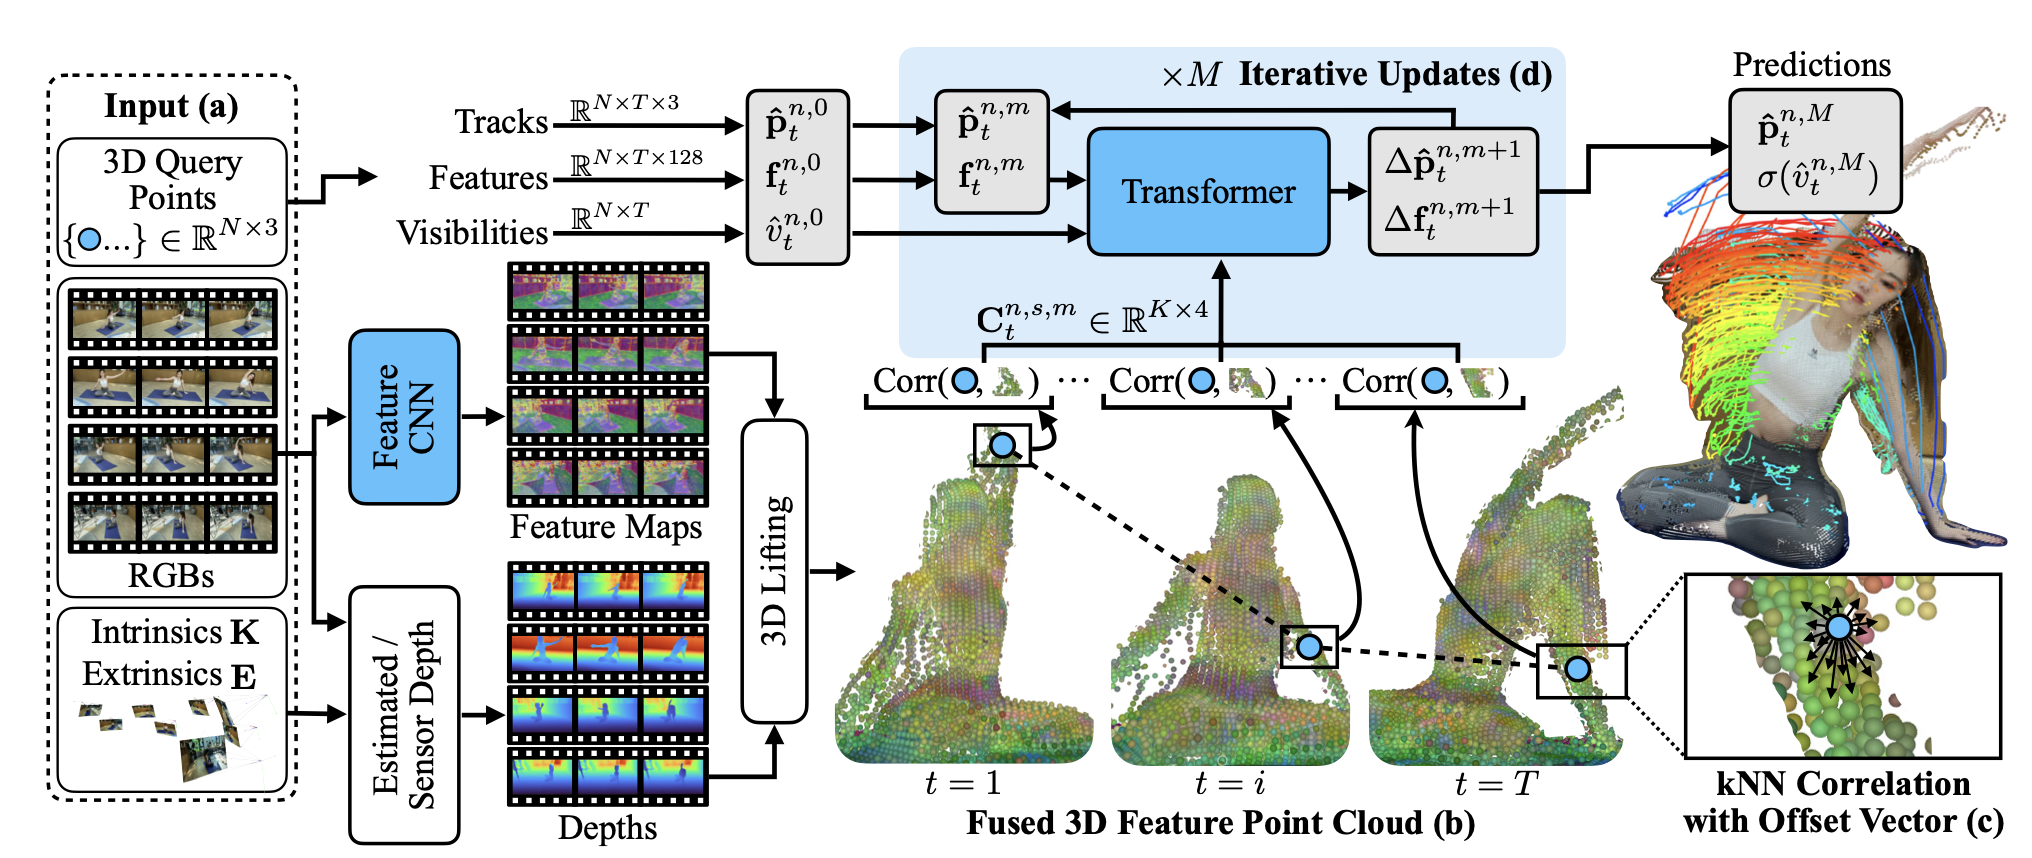
\includegraphics[width=\textwidth]{images/mvtracker_original_pipeline.png}
    \caption{MVTracker pipeline (from \cite{rajic2025multiview3dpointtracking}). \textbf{(a)} Given synchronized multi-view RGB videos with known intrinsics and extrinsics, per-view feature maps are extracted using a CNN-based encoder. \textbf{(b)} A point cloud is constructed from estimated or sensor-based depth maps, associating each point with learned feature embeddings. \textbf{(c)} Directed kNN-based correlation within the point cloud captures spatiotemporal relationships across views. \textbf{(d)} A transformer-based update module iteratively refines point trajectories using self-attention over multi-view feature correlations within a sliding temporal window. The blue blocks denote trainable neural models. The visualized sequence is from SelfCap \cite{Xu2024SelfCap} and uses DUSt3R \cite{wang2024dust3rgeometric3dvision} to estimate depth.}
    \label{fig:mvtracker_pipeline}
\end{figure}

\section{Dense 3D Reconstruction via Point Map Regression}
The depth maps that feed MVTracker's point cloud can be generated by a variety of methods; the following three sections cover the reconstruction and correspondence systems most relevant to this pipeline.

DuSt3R \cite{wang2024dust3rgeometric3dvision} represents a paradigm shift in 3D reconstruction by casting the problem as a direct regression of dense point maps from image pairs, bypassing the traditional pipeline of feature matching, essential matrix estimation, and triangulation. Built on standard Transformer encoders and decoders, DuSt3R shares information between views through cross-attention and leverages pre-trained vision weights to learn strong geometric and shape priors.

A key property of DuSt3R is its agnosticism to camera parameters: the method requires no prior knowledge of camera intrinsics or extrinsic poses and can even perform monocular reconstruction from a single input image. For multi-image collections, a fast global alignment procedure expresses all pairwise point maps in a common reference frame, effectively stitching the scene together in 3D space.

However, DuSt3R assumes static scenes, relying on overlapping visual content across views to establish correspondences. It does not explicitly model moving or articulated objects such as humans, which limits its direct applicability to dynamic human-centric scenarios.

\section{Grounding Image Matching in 3D with MASt3R}
MASt3R \cite{mast3r_arxiv24} builds upon DuSt3R by adding a dedicated head that regresses dense local feature maps alongside the 3D point maps. While 3D regression is inherently noisy, these learned features enable highly accurate, pixel-level correspondences that go beyond what point map regression alone can provide.

To handle high-resolution images, MASt3R adopts a coarse-to-fine strategy: it first matches downscaled image versions to establish coarse correspondences, then uses a greedy window-sampling approach to zoom in on overlapping areas at full resolution for fine-grained matching. This is complemented by Fast Reciprocal Matching (FRM), a sub-sampling algorithm that iterates through mutual nearest neighbours rather than exhaustively comparing every pixel. FRM reduces the quadratic $O(W^2 H^2)$ complexity by nearly two orders of magnitude and actually improves pose accuracy by filtering out outliers.

A central design choice is the 3D-aware loss function: MASt3R combines the standard 3D regression loss with a matching loss (InfoNCE) that grounds feature learning in 3D geometry, ensuring that the network is specifically rewarded for identifying exact pixel correspondences. This grounding in 3D makes the learned features geometrically consistent rather than purely appearance-based.

For human-centric tracking, this selective matching capability is particularly relevant. In multi-view human scenes, the background dominates the image while the subject of interest occupies a relatively small region. MASt3R's coarse-to-fine and reciprocal matching mechanisms provide a natural way to focus correspondence estimation on the regions that matter---the tracked human---rather than wasting capacity on background detail. The approach in this thesis pursues a complementary strategy (Chapter~\ref{ch:method}): rather than filtering correspondences, we enrich the point cloud itself with dense human body surface geometry so that the downstream kNN correlation naturally attends to body-relevant regions.

\section{Continuous 3D Reconstruction for Video with CuT3R}
CuT3R \cite{wang2025continuous3dperceptionmodel} extends the DuSt3R/MASt3R line of work from static image pairs to live video streams, introducing a framework for continuous tracking and 3D reconstruction. Rather than processing frames in isolation or as an unordered set, CuT3R maintains a persistent 3D memory state --- represented as a set of latent tokens --- that is updated incrementally as new frames arrive. This allows the model to retain geometric knowledge of scene regions that have left the current field of view.

The system operates through two complementary functions. An \textit{Update} function integrates new visual information into the memory tokens, while a \textit{Query} (Get) function extracts the current 3D point map and camera pose from the stored state. Each incoming frame is encoded with a Vision Transformer (ViT); the memory update is not a simple vector addition but uses Transformer decoders with cross-attention, allowing the memory state to attend to the new image tokens and fuse temporal history with current observations.

For the human tracking setting, CuT3R's persistent state mechanism is conceptually relevant: occlusion and re-entry are precisely the scenarios where a model that remembers prior geometry has an advantage over one that reconstructs from the current frame alone. However, CuT3R targets general scene reconstruction and does not explicitly model articulated motion, which remains the domain of body-specific representations such as SMPL.

\section{Human Body Models: SMPL and MHR}
\label{sec:smpl}
Parametric body models provide a compact, differentiable representation of human shape and pose. SMPL \cite{loper2015smpl} (Skinned Multi-Person Linear Model) represents the body as a function of two parameter sets: shape parameters $\boldsymbol{\beta} \in \mathbb{R}^{10}$, which encode identity-specific body proportions, and pose parameters $\boldsymbol{\theta} \in \mathbb{R}^{72}$, which encode the joint rotation angles. Given $(\boldsymbol{\beta}, \boldsymbol{\theta})$, SMPL produces a triangulated mesh of 6,890 vertices and 13,776 faces. Critically, the mesh is fully deterministic and differentiable with respect to both parameter sets, making it amenable to fitting by gradient descent against image evidence.

The Mesh Human Representation (MHR) extends the standard skeleton beyond the 17-joint COCO convention to 70 joints, adding detailed coverage of the hands (finger joints) and feet. This richer joint set allows body-part labels to be assigned at the level of individual fingers and toes, which is relevant when tracking hand-object interaction scenes such as those in DexYCB.

\section{SAM-3D-Body}
\label{sec:sam3d}
SAM-3D-Body \cite{sam3dteam2025sam3d3dfyimages} is a per-frame, per-view human mesh recovery system that fits SMPL to monocular image crops. Given an input frame, it produces: 70 MHR joint positions in camera space ($\mathbf{p}_{\text{joints}} \in \mathbb{R}^{70 \times 3}$), the full SMPL mesh vertex set ($\mathbf{V} \in \mathbb{R}^{6890 \times 3}$), pose and shape parameters ($\boldsymbol{\theta}, \boldsymbol{\beta}$), and a camera-frame translation vector. The joints define a compact semantic scaffold over the body that can be used to measure whether two candidate points are likely to correspond to similar anatomical regions, even under viewpoint changes or temporary occlusions. The mesh vertices provide dense surface coverage of the entire body, including regions that are systematically under-represented in depth maps.

\section{Multi-View Fusion via Entropy Weighting}
\label{sec:mvsam3d}
MV-SAM3D \cite{li2026mvsam3dadaptivemultiviewfusion} addresses a challenge common to multi-view systems: not all views contribute equally to a given spatial location. In a multi-view 3D generation setting, MV-SAM3D observes that na\"ively averaging latent representations across views produces blurred geometry because occluded or ambiguous views dilute confident ones. Their solution is an entropy-weighted fusion scheme with two passes:

\begin{enumerate}
    \item \textbf{Warmup pass.} A single denoising step is run with simple view averaging. Cross-attention patterns are collected for each latent position and each view.
    \item \textbf{Entropy computation.} For each latent position $i$ and view $v$, the Shannon entropy of the attention distribution over image patches is computed:
    \begin{equation}
        H_v(i) = -\sum_j p_{ij} \log p_{ij},
    \end{equation}
    where $p_{ij}$ is the normalised attention weight from latent $i$ to patch $j$. Low entropy indicates the view attends confidently to a specific image region; high entropy indicates diffuse, uncertain attention.
    \item \textbf{Weighted fusion.} Per-view weights are derived via a temperature-scaled softmax over inverted entropies:
    \begin{equation}
        w_v(i) = \frac{\exp(-\alpha \cdot H_v(i))}{\sum_{v'} \exp(-\alpha \cdot H_{v'}(i))},
    \end{equation}
    with $\alpha$ controlling sharpness (typically 30--60). The fused latent is then $\mathbf{z}(i) = \sum_v w_v(i) \cdot \mathbf{z}_v(i)$.
\end{enumerate}

Although MV-SAM3D operates in a generative diffusion setting rather than point tracking, the core insight --- that multi-view fusion should be confidence-weighted rather than uniform --- transfers directly. In Chapter~\ref{ch:method}, we adapt this principle to the point cloud augmentation pipeline: instead of averaging CNN features equally across views when computing mesh vertex descriptors, we weight each view's contribution by a geometric confidence signal (depth consistency), ensuring that occluded or unreliable views do not corrupt the fused feature.

% --- Chapter 3: Methodology ---
\chapter{SAM3D-Enhanced MV-Tracker}
\label{ch:method}
\section{Overview}
The central challenge in applying MVTracker to human-centric scenes is that the depth-based point cloud --- the sole source of correlation evidence --- is frequently incomplete over human bodies. Reflective or textured clothing, thin limbs, and self-occlusion all produce holes and noise in the depth map, leaving the kNN correlation search without valid candidates near the tracked body surface.

This chapter presents point cloud augmentation as the primary technical contribution: directly inserting SMPL mesh vertices from SAM3D into the depth-based point cloud (Section~\ref{sec:pc_aug}), providing dense geometric coverage where depth is unreliable. Section~\ref{sec:knn_bias} describes an earlier kNN semantic bias approach that was evaluated and found ineffective, motivating the shift to direct geometric augmentation. Both strategies preserve full backward compatibility with the baseline MVTracker architecture.

Figure~\ref{fig:architecture} provides an architectural overview of the augmented MVTracker pipeline. The key modification (highlighted in the lower-left) is the addition of SAM3D mesh vertices to the fused 3D feature point cloud. These vertices are projected into each camera view to extract CNN features via bilinear sampling, then aggregated with depth-weighted multi-view fusion. The augmented point cloud (depth points + mesh vertices) feeds into the standard kNN correlation and iterative transformer updates, requiring no changes to the downstream architecture.

\begin{figure}[htbp]
    \centering
    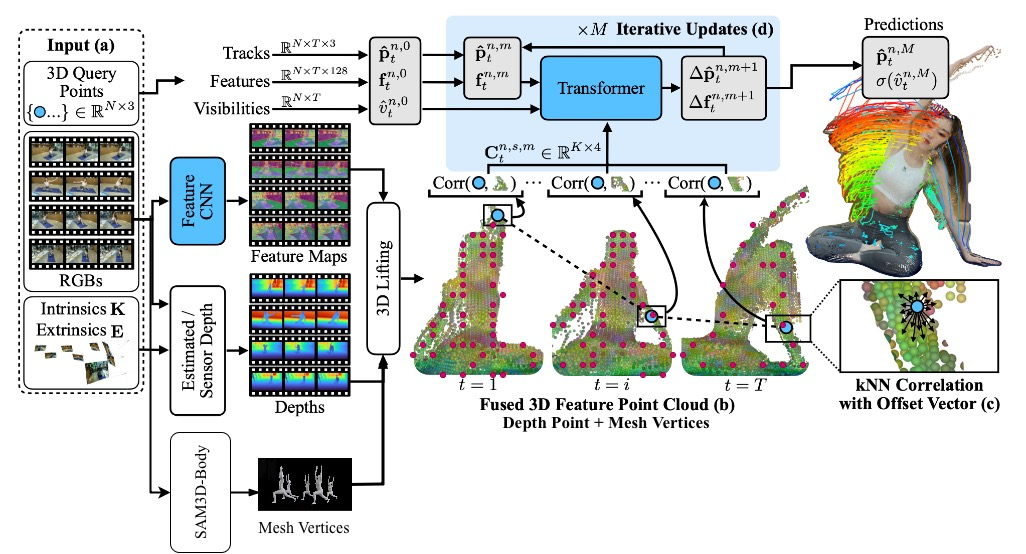
\includegraphics[width=\textwidth]{images/mesh_vertices_aug_mvtracker.jpg}
    \caption{Architecture overview of MVTracker with SAM3D mesh vertex augmentation. \textbf{(a)} Multi-view RGB inputs with camera parameters. \textbf{(b)} The fused 3D feature point cloud now includes both depth-based points ($\sim$57k, from back-projected depth maps) and SAM3D mesh vertices ($\sim$7k per person, from SMPL body model fits). Mesh vertex features are obtained by projecting vertices into each camera view, bilinearly sampling the CNN feature maps, and computing a depth-weighted average across views. \textbf{(c)} kNN correlation operates on the augmented point cloud, providing body-surface neighbours even where depth is missing. \textbf{(d)} The transformer iteratively refines 3D track positions and features, unchanged from the baseline.}
    \label{fig:architecture}
\end{figure}

\section{Point Cloud Augmentation with Mesh Vertices}
\label{sec:pc_aug}

\subsection{Mechanism}
The point cloud augmentation approach concatenates SAM3D SMPL mesh vertices directly into the depth-based point cloud before the kNN correlation search. This means that even where the depth sensor provides no coverage, the tracker can find body-surface points as nearest neighbours and compute meaningful correlations from them.

SAM-3D-Body \cite{sam3dteam2025sam3d3dfyimages} produces approximately 6,890 SMPL \cite{loper2015smpl} mesh vertices per detected person per frame in world coordinates. These are appended to the existing depth-based point cloud ($\sim$57k points) at each pyramid level, representing a $\sim$12\% increase in cloud size with modest computational overhead.

\subsection{Feature Extraction for Mesh Vertices}
Depth-based points carry 128-dimensional CNN feature vectors obtained by lifting 2D image features into 3D. Mesh vertices have no direct depth pixel to sample from, so their features are computed by multi-view projection:
\begin{enumerate}
    \item Each mesh vertex $\mathbf{v}$ is projected into every camera view using the known extrinsics and intrinsics.
    \item The CNN feature map is bilinearly sampled at the projected pixel location for each view where the vertex projects within image bounds.
    \item Features are averaged across all valid views to produce the final 128-d feature vector for that vertex.
\end{enumerate}
This gives each mesh vertex a geometrically grounded appearance descriptor consistent with those of the surrounding depth points, requiring no new learnable parameters.

\subsection{Depth-Weighted Multi-View Feature Fusion}
\label{sec:depth_weighted_fusion}
The simple averaging scheme described above treats all views equally when computing mesh vertex features. However, a vertex that is occluded in a given view --- for instance, because the person's arm is between the vertex and the camera --- will produce a feature sampled from the occluding surface rather than from the vertex's true appearance. Inspired by the entropy-weighted fusion in MV-SAM3D \cite{li2026mvsam3dadaptivemultiviewfusion} (Section~\ref{sec:mvsam3d}), we replace uniform averaging with a confidence-weighted scheme that requires no learnable parameters.

For each mesh vertex $\mathbf{v}$ projected into view $v$, we compare the projected depth $z_{\text{proj}}$ (the vertex's distance from the camera) against the depth map value $z_{\text{map}}$ sampled at the projected pixel location. If the depth map records a closer surface ($z_{\text{map}} \ll z_{\text{proj}}$), the vertex is likely occluded in that view. The per-view weight is:
\begin{equation}
    w_{\text{depth}}(v) = \exp\!\left(-\alpha_d \left\lvert 1 - \frac{z_{\text{map}}}{z_{\text{proj}}} \right\rvert\right),
\end{equation}
where $\alpha_d$ controls sharpness (default 15.0). When $z_{\text{map}} \approx z_{\text{proj}}$ (the vertex is at the visible surface), $w_{\text{depth}} \approx 1$; when they diverge significantly, $w_{\text{depth}} \to 0$. For pixels where the depth map is invalid (zero or missing), the weight falls back to 1.0 (unweighted).

The fused feature vector for vertex $\mathbf{v}$ is then the weighted mean:
\begin{equation}
    \mathbf{f}(\mathbf{v}) = \frac{\sum_{v \in \mathcal{V}_{\text{vis}}} w_{\text{depth}}(v) \cdot \mathbf{f}_v(\mathbf{v})}{\sum_{v \in \mathcal{V}_{\text{vis}}} w_{\text{depth}}(v)},
\end{equation}
where $\mathcal{V}_{\text{vis}}$ is the set of views where the vertex projects within image bounds with positive depth.

An optional second pass implements feature consensus weighting, analogous to MV-SAM3D's two-pass warmup-then-refine approach. After computing the depth-weighted mean $\bar{\mathbf{f}}$, each view's feature is compared to the consensus via cosine similarity:
\begin{equation}
    w_{\text{cons}}(v) = \exp\!\left(\alpha_f \cdot \frac{\mathbf{f}_v \cdot \bar{\mathbf{f}}}{\lVert \mathbf{f}_v \rVert \lVert \bar{\mathbf{f}} \rVert}\right),
\end{equation}
with $\alpha_f = 5.0$. The final weight combines both signals: $w(v) = w_{\text{depth}}(v) \cdot w_{\text{cons}}(v)$. This ensures that views which are both geometrically consistent and produce features in agreement with other views receive the highest weight.

Since all weights are derived from geometry and feature statistics (no learnable parameters), the depth-weighted fusion operates zero-shot with the pretrained MVTracker checkpoint, avoiding the catastrophic forgetting observed during finetuning.

Figure~\ref{fig:depth_weighted_fusion} illustrates the depth-weighted fusion mechanism. Each mesh vertex is projected into all camera views; depth consistency is checked by comparing the vertex's projected depth ($z_{\text{proj}}$) against the depth map value ($z_{\text{map}}$) at the projected pixel location. Views where the vertex is occluded (large depth mismatch) receive near-zero weight, while visible views dominate the final feature aggregation. In the example shown, Views 1 and 7 are visible (weights 0.68 and 0.65), View 20 is fully occluded (weight 0.00), and View 14 is partially occluded (weight 0.08). The weighted aggregation $\sum f \ast w / \sum w$ produces a 128-dimensional feature vector that is robust to occlusion.

\begin{figure}[htbp]
    \centering
    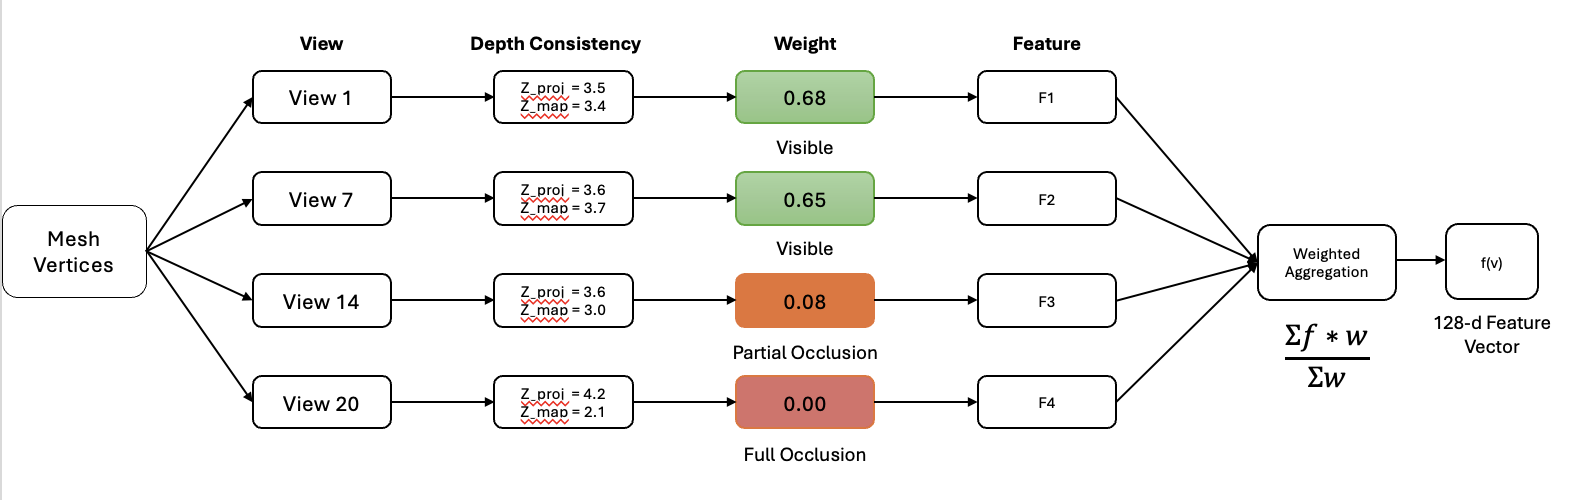
\includegraphics[width=0.95\textwidth]{images/depth_weighted_fusion_manual.png}
    \caption{Depth-weighted multi-view fusion for mesh vertex features. Each mesh vertex is projected into 4 camera views. For each view, depth consistency is evaluated by comparing projected depth $z_{\text{proj}}$ (vertex distance to camera) against depth map value $z_{\text{map}}$ (sensor reading at projected pixel). Consistent depths (green, $z_{\text{map}} \approx z_{\text{proj}}$) indicate visibility and receive high weights (0.65--0.68). Large depth mismatches indicate occlusion: partial occlusion (orange) receives low weight (0.08), full occlusion (red, $z_{\text{map}} \ll z_{\text{proj}}$) receives near-zero weight (0.00). The weighted mean $\sum f \ast w / \sum w$ produces a robust 128-d feature vector dominated by visible views, ensuring occluded projections do not corrupt the descriptor.}
    \label{fig:depth_weighted_fusion}
\end{figure}

\subsection{Backward Compatibility}
The forward pass accepts an optional tensor \texttt{sam3d\_vertices\_world} of shape $(B, T, n_{\text{persons}}, V, 3)$, where $V \approx 6890$. When this tensor is absent, the augmentation step is skipped and the model behaves identically to the baseline MVTracker. The fusion mode is configurable: \texttt{mean} reproduces the original uniform averaging, \texttt{depth\_weighted} enables depth-consistency weighting, and \texttt{consensus} adds the two-pass feature consensus refinement. The kNN bias code (Section~\ref{sec:knn_bias}) remains in the codebase and can be combined with augmentation, but the primary experiments evaluate augmentation alone.

\section{Motivating Negative Result: kNN Semantic Bias}
\label{sec:knn_bias}

\subsection{Mechanism}
Rather than changing the point cloud, the kNN bias approach re-ranks the neighbour candidates used for correlation. For each query point, instead of fetching $k=16$ nearest neighbours in Euclidean space, we over-fetch $k' = 4k = 64$ candidates and then re-rank them using a combined spatial-semantic distance.

For each candidate, a soft body-part assignment is computed based on its distance to the 70 MHR joints provided by SAM3D:
\begin{equation}
    \mathbf{w} = \operatorname{softmax}\left( -\frac{\mathbf{d}_{\text{joint}}}{\tau} \right),
\end{equation}
where $\tau$ is a learnable temperature parameter (initialised to 0.15). The semantic distance between a query point $q$ and a candidate $c$ is then
\begin{equation}
    d_{\text{sem}} = \lVert \mathbf{w}_{q} - \mathbf{w}_{c} \rVert_2,
\end{equation}
and the combined ranking criterion is
\begin{equation}
    d_{\text{adj}} = d_{\text{spatial}} + |\lambda|\, d_{\text{sem}},
\end{equation}
where $\lambda$ is a learnable strength parameter (initialised to 0.1). Top-$k$ selection is performed on $d_{\text{adj}}$. To provide a differentiable gradient path to $\lambda$ and $\tau$, a soft weighting
\begin{equation}
    \omega = \exp\!\left(-\frac{|\lambda|\, d_{\text{sem}}}{\tau + 10^{-6}}\right)
\end{equation}
is applied element-wise to the selected correlation features.

\subsection{Limitations and Depth-Dependent Behaviour}
Under near-perfect Dynamic3DGS depth, the kNN bias approach produced no measurable improvement in tracking quality, motivating the shift to point cloud augmentation as the primary approach. The reasoning was that re-ranking operates only on candidates that already exist in the depth-based point cloud: where the depth map has holes, there are no good candidates regardless of ranking criterion.

However, subsequent evaluation with noisy DUSt3R depth (Section~\ref{sec:duster_results}) revealed that kNN bias \emph{does} help when the point cloud is spatially inaccurate. With DUSt3R depth, re-ranking by body-part semantic proximity compensates for spatial errors in the point cloud, steering the correlation search toward anatomically plausible neighbours. This produced the best narrow-baseline result of any zero-shot method (+2.12 AJ over baseline). The depth-dependent behaviour is instructive: with perfect depth, spatial kNN already finds optimal neighbours, and semantic re-ranking adds only noise; with noisy depth, spatial neighbours are unreliable, and semantic guidance provides a useful corrective signal.

% --- Chapter 4: Data Generation & Training ---
\chapter{The Synthetic-to-Real Data Engine}
\label{ch:data}
\section{Pipeline Overview}
Inspired by AnthroTAP \cite{kim2026anthrotaplearningpointtracking}, we implement a multi-stage offline data engine to produce MVTracker-compatible human trajectory supervision from Panoptic Studio \cite{joo2015panoptic} data.

\textbf{Stage 1: Per-view SAM3D inference.} SAM-3D-Body is run independently on each camera stream to produce per-frame 3D keypoints (70 MHR joints), mesh vertices, pose and shape parameters, and camera-frame translations.

\textbf{Stage 2: Cross-view fusion and trajectory generation.} Camera-space predictions are transformed to world coordinates using Panoptic extrinsics. Persons are associated across views by pelvis proximity via the Hungarian algorithm, then joints and vertices are averaged across associated views. A temporal uniform filter smooths trajectories. The pipeline samples both joints and mesh vertices as track points and computes per-view visibility using projection validity, image-bounds checks, and depth-based occlusion tests.

\textbf{Stage 3: Export.} The output is stored as \texttt{human\_tracks.npz} files with fields aligned to MVTracker datapoints: \texttt{trajectory\_3d}, \texttt{visibility}, \texttt{query\_points\_3d}, and \texttt{valid}, plus metadata such as number of persons, keypoints, and track types.

\section{Dataset Integration}
A dedicated \texttt{PanopticHumanTrajectoryDataset} loader ingests generated tracks and returns both the standard trajectory tensors and \texttt{sam3d\_vertices\_world} --- the per-frame SMPL mesh vertex positions in world space --- which are used by the point cloud augmentation module at training and inference time.

The same scene normalisation used by the baseline Panoptic loader is applied to both trajectories and SAM3D outputs (scale 2.5 and $-90^{\circ}$ rotation around the X-axis), ensuring consistent coordinate frames. Camera-space outputs from SAM3D are transformed to Panoptic world coordinates through
\begin{equation}
    \mathbf{p}_{\text{world}} = \mathbf{R}^{-1} (\mathbf{p}_{\text{cam}} - \mathbf{t}).
\end{equation}

\section{Training Strategy}
Since the point cloud augmentation approach introduces no new learnable parameters, the full MVTracker backbone is available for optimisation. Training starts from a pre-trained MVTracker checkpoint (trained for 200k steps on Kubric synthetic data) and continues with the augmented point cloud on Panoptic human sequences.

Loss definitions remain unchanged from baseline MVTracker: a trajectory regression loss and a balanced visibility BCE loss. Optimisation uses AdamW with OneCycleLR. The augmentation is active throughout training, so the model learns correlation features over a point cloud that includes both depth points and SAM3D mesh vertices from the first training step.

A preliminary run of 5,000 steps on only four Panoptic training sequences exhibited catastrophic forgetting: average AJ across the three evaluation configurations dropped from 56.14 to 31.47. Increasing the training set to all $\sim$55 valid sequences (filtering empty-room sequences via a \texttt{track\_valid} check in the dataset loader) and extending training to 20,000 steps did not resolve the forgetting: average AJ fell further to 27.68. The learning rate ($5 \times 10^{-4}$, identical to the Kubric pretraining schedule) is identified as the primary cause --- it is too aggressive for finetuning a strong pretrained backbone on a new domain. The zero-shot augmented model therefore serves as the primary reported result (Section~\ref{sec:summary_findings}).

% --- Chapter 5: Experiments & Results ---
\chapter{Evaluation}
\label{ch:eval}
\section{Evaluation Protocol}
\subsection{Metrics}
We evaluate with the standard 3D point-tracking metrics used by MVTracker: 3D Average Jaccard (AJ), Average Trajectory Error (ATE), Median Trajectory Error (MTE), Final Displacement Error (FDE), thresholded point accuracy ($\delta$ at 0.05, 0.10, 0.20, 0.40), occlusion accuracy, and survival rate.

\subsection{Configurations}
We use three configurations for controlled comparison: (i) baseline MVTracker with depth-only point cloud, (ii) MVTracker with kNN semantic bias (zero-shot, no finetuning), and (iii) MVTracker with point cloud augmentation (with and without finetuning on Panoptic human data).

All configurations are evaluated on the same three Panoptic view setups:
\begin{itemize}
    \item \texttt{panoptic-human-views1\_7\_14\_20}
    \item \texttt{panoptic-human-views27\_16\_14\_8}
    \item \texttt{panoptic-human-views1\_4\_7\_11}
\end{itemize}
A dedicated comparison script computes per-dataset deltas between baseline and augmented runs.

\subsection{Training Setup}
All finetuning runs restore from the pretrained Kubric checkpoint (\texttt{mvtracker\_200000\_june2025.pth}, 200k steps). Each training step processes one sequence of 24 frames with 384 sampled tracks in bf16-mixed precision. SAM3D SMPL mesh vertices ($\sim$6{,}890 per person) are concatenated into the point cloud at each pyramid level throughout training. The key variables across finetuning configurations are: learning rate ($5 \times 10^{-4}$ to $1 \times 10^{-5}$), whether the CNN encoder is frozen, the number of training sequences (4--16), the depth source (Dynamic3DGS or DUSt3R), and the active SAM3D interventions. These are detailed per configuration in Section~\ref{sec:finetuning_analysis}.

\section{Depth Source Analysis and Contamination}
\label{sec:depth_contamination}

A critical finding emerged during evaluation: the six TAPVid-3D benchmark sequences (basketball, boxes, football, juggle, softball, tennis) use \textbf{Dynamic 3D Gaussian Splatting} \cite{luiten2023dynamic} depth maps as input. Dynamic3DGS is not a depth estimation method but rather a scene reconstruction technique that fits 3D Gaussians to \emph{all 31 camera views} of each sequence via multi-view optimization. The resulting depth maps are then rendered from the fitted Gaussian model.

This creates a methodological issue: the depth maps used as input (X) are derived from the same multi-view imagery we are attempting to track (Y). Dynamic3DGS depths represent near-perfect geometry because they encode information from all views, effectively providing the tracker with ground-truth 3D structure. Evaluating with these depths inflates performance and obscures the true value of SAM3D mesh augmentation --- when the depth-based point cloud already covers human bodies accurately, there is little room for mesh vertices to contribute.

\subsection{Zero-Depth Ablation Study}

To quantify MVTracker's dependence on depth and isolate the contribution of SAM3D mesh augmentation, we conducted an ablation study comparing performance with and without depth on the same six sequences. Table~\ref{tab:ablation_results} reports results under two depth conditions (Dynamic3DGS and zero) crossed with two augmentation conditions (no SAM3D and with SAM3D mesh vertices).

\begin{table}[htbp]
    \centering
    \resizebox{\textwidth}{!}{%
    \begin{tabular}{lccccccccc}
        \toprule
        & \multicolumn{3}{c}{\texttt{views1\_7\_14\_20}} & \multicolumn{3}{c}{\texttt{views27\_16\_14\_8}} & \multicolumn{3}{c}{\texttt{views1\_4\_7\_11}} \\
        \cmidrule(lr){2-4} \cmidrule(lr){5-7} \cmidrule(lr){8-10}
        Configuration & AJ & $\delta^{0.10}$ & ATE & AJ & $\delta^{0.10}$ & ATE & AJ & $\delta^{0.10}$ & ATE \\
        \midrule
        \multicolumn{10}{l}{\textit{With Dynamic3DGS depth (near-perfect)}} \\
        \quad Baseline          & 55.29 & 59.62 & 16.39 & 56.67 & 61.39 & 16.12 & 54.92 & 50.98 & 14.18 \\
        \quad + SAM3D mesh      & 56.48 & 60.94 & 15.72 & 56.66 & 61.47 & 15.57 & 55.27 & 51.04 & 13.72 \\
        \midrule
        \multicolumn{10}{l}{\textit{Without depth (zeros)}} \\
        \quad Baseline          & 9.75 & 9.24 & 61.41 & 5.67 & 6.87 & 111.63 & 22.29 & 13.54 & 45.73 \\
        \quad + SAM3D mesh      & 9.77 & 9.29 & 61.33 & 5.68 & 6.88 & 111.97 & 22.29 & 13.55 & 45.70 \\
        \bottomrule
    \end{tabular}}
    \caption{Ablation study comparing Dynamic3DGS depth vs zero depth with and without SAM3D mesh augmentation. Dynamic3DGS depths are near-perfect (trained on test scenes), while zero depth forces the model to rely solely on RGB features and camera geometry. All numbers are percentages except ATE (mm). Mesh augmentation provides minimal benefit with perfect depth (+0.5 AJ average) and no benefit without depth (+0.01 AJ average).}
    \label{tab:ablation_results}
\end{table}

\section{Analysis}

\subsection{The Depth Dependency}
Table~\ref{tab:ablation_results} reveals that MVTracker is \emph{almost entirely dependent} on depth-based geometry. When Dynamic3DGS depth is removed and replaced with zeros, average 3D Average Jaccard drops from 55.63 to 12.57 --- a 77\% relative degradation. Tracking error (ATE) increases from 15.5\,mm to 73.0\,mm on average, and within-10\,cm accuracy collapses from 58\% to 10\%. Without depth, the depth-based point cloud contains no points, leaving the kNN correlation search with no valid neighbours and no spatial evidence for the transformer to process.

This dependence is expected: the pretrained MVTracker checkpoint was trained for 200k steps on Kubric synthetic data with ground-truth depth. The model has learned to rely on dense, view-specific 3D features sampled from depth-lifted CNN activations. RGB-only tracking (with camera poses but no depth) is a fundamentally different problem that would require training from scratch or extensive domain adaptation.

An apparent anomaly in Table~\ref{tab:ablation_results} is that the zero-depth average (12.57\%) exceeds the DUSt3R average (9.07\%) reported later in Table~\ref{tab:duster_results}, seemingly implying that no depth is better than estimated depth. This is a statistical artifact from unequal configuration difficulty. On two wide-baseline configurations (\texttt{views1\_7\_14\_20} and \texttt{views27\_16\_14\_8}), DUSt3R outperforms zero depth by 1.8--2.2 AJ points, as expected. However, on the narrow-baseline configuration \texttt{views1\_4\_7\_11}, zero depth scores 22.29\% while DUSt3R scores only 7.76\% --- a 14.5-point reversal. The narrow-baseline cameras (span of 10 camera indices vs 19 for wide baselines) have small viewpoint changes, making RGB-based appearance matching more effective. Crucially, DUSt3R's depth estimates have highest uncertainty on narrow baselines due to poor triangulation geometry, and the resulting noisy depth \emph{actively misleads} the point cloud construction. Bad depth is worse than no depth for this specific configuration. The zero-depth score on \texttt{views1\_4\_7\_11} (22.29\%) is an outlier that dominates the average; it does not indicate that zero depth is generally superior to estimated depth.

Figure~\ref{fig:depth_contamination} illustrates the performance inflation from using optimization-based reconstruction depths (Dynamic3DGS) rather than online-estimable depths (DUSt3R): baseline tracking degrades by $6\times$ when realistic depth is used, confirming that the TAPVid-3D benchmark evaluation does not reflect deployable system performance.

\begin{figure}[htbp]
    \centering
    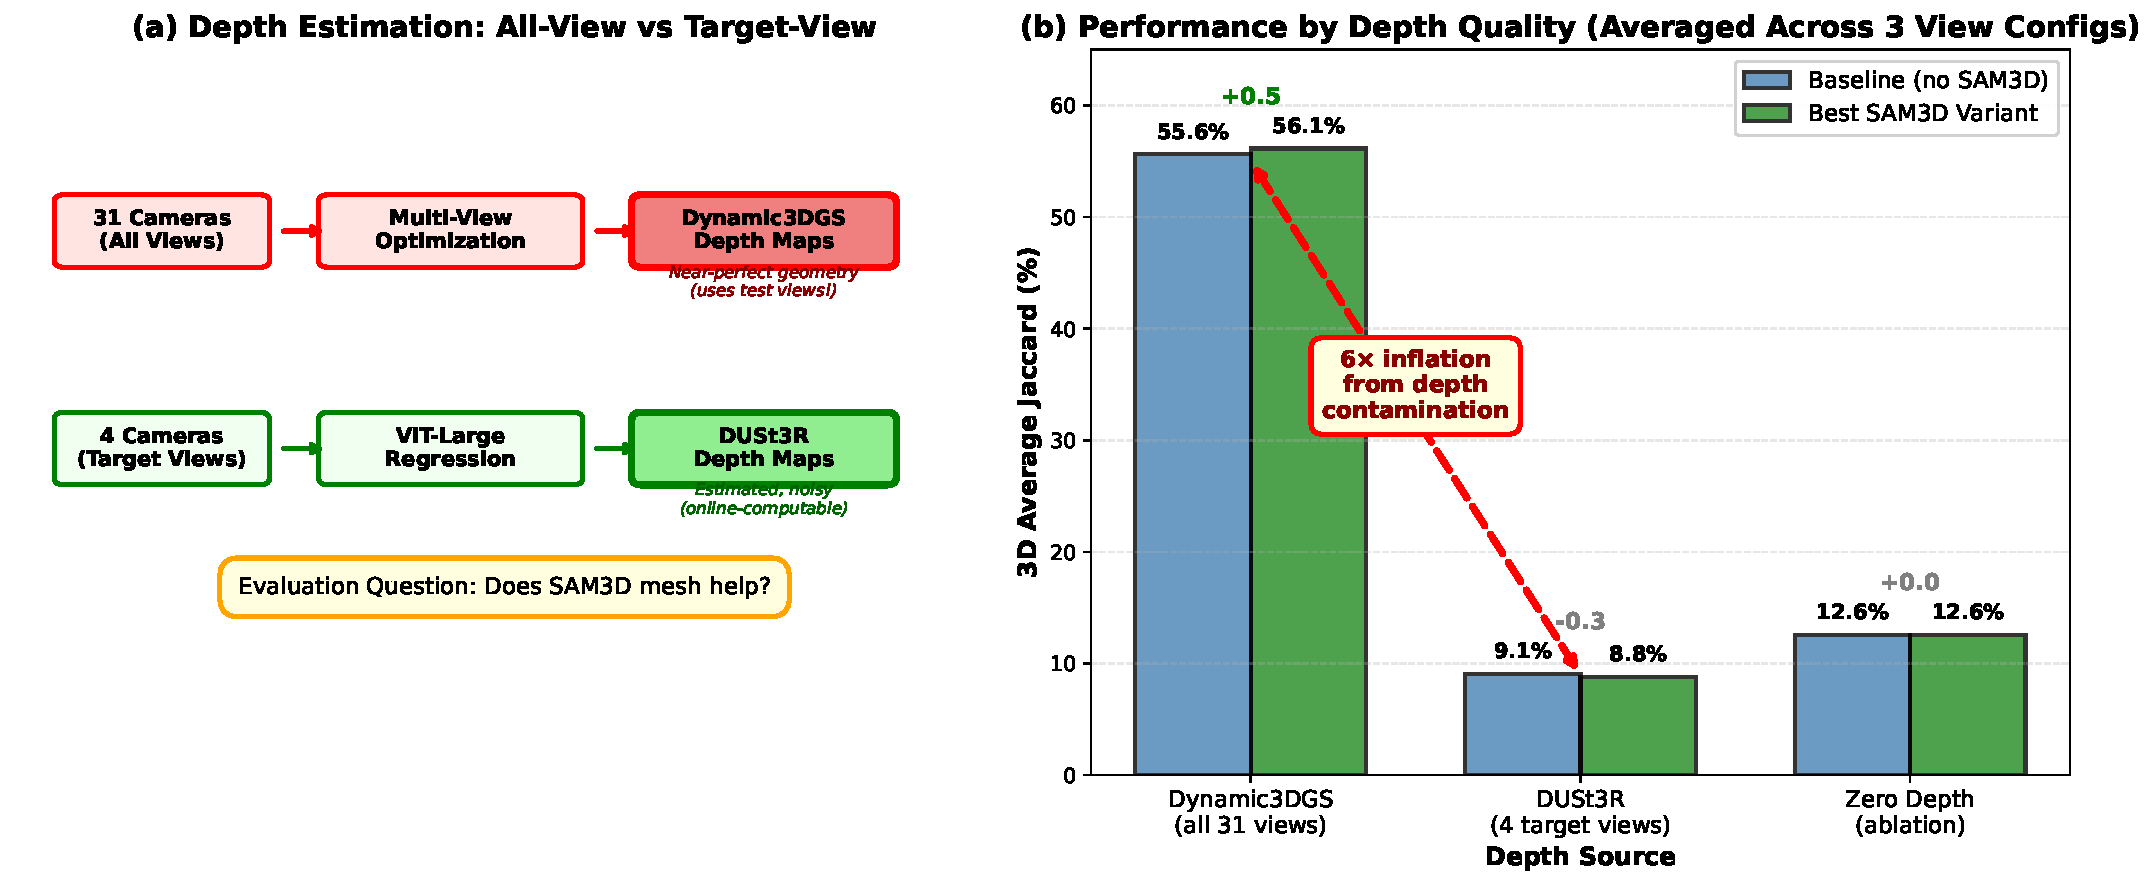
\includegraphics[width=\textwidth]{images/depth_contamination.pdf}
    \caption{Depth source contamination analysis. \textbf{(a)} Dynamic3DGS uses multi-view optimization on all 31 cameras (including test views), producing near-perfect geometry. DUSt3R estimates depth from only 4 target cameras, producing noisy but online-computable depth. \textbf{(b)} Baseline MVTracker performance by depth source. Dynamic3DGS inflates results by $6\times$ relative to realistic DUSt3R depth. The best SAM3D variant (kNN semantic bias) improves DUSt3R performance by +0.6 AJ average, with negligible effect under perfect or absent depth.}
    \label{fig:depth_contamination}
\end{figure}

\subsection{SAM3D Mesh Augmentation: Minimal Effect Under Both Conditions}
SAM3D mesh vertex augmentation produces negligible improvements regardless of depth availability. With Dynamic3DGS depth, adding ~500 SMPL mesh vertices to the existing 57k-point depth cloud increases average AJ by only 0.5 points (from 55.63 to 56.14). The depth-based geometry already covers human bodies accurately, leaving little room for mesh vertices to contribute --- they represent less than 1\% of the total point cloud, so kNN queries ($k=16$) rarely select mesh vertices as neighbours.

Without depth, mesh augmentation similarly provides no benefit: average AJ increases from 12.57 to 12.58 (+0.01 points). Although the mesh vertices now constitute a larger fraction of the (nearly empty) point cloud, their features are computed via multi-view projection and averaging, which produces ``blurred'' appearance descriptors that differ statistically from the view-specific depth-based features the pretrained transformer expects. Attempts to increase mesh density (5,000 vertices instead of 500) and preserve view-specific features (concatenating per-view mesh vertices without averaging) both degraded performance further, confirming that the pretrained model cannot effectively utilize mesh-based features without retraining.

\subsection{The Role of Depth Quality: Dynamic3DGS vs DUSt3R}
\label{sec:duster_results}
The evaluation protocol described above uses Dynamic3DGS depths, which are fitted to all 31 camera views via multi-view optimization and thus represent near-ground-truth geometry. This is appropriate for establishing an upper bound on performance but does not reflect realistic deployment scenarios where depth must be estimated online from the target views alone. The original MVTracker paper evaluates with DUSt3R \cite{wang2024dust3rgeometric3dvision} --- a learning-based depth estimator that processes only the selected camera views --- to assess robustness to imperfect depth.

Table~\ref{tab:duster_results} reports results with DUSt3R-estimated depths. DUSt3R depths were generated per-frame for each 4-view configuration using the ViT-Large model at 512$\times$288 resolution with 300 global alignment iterations.

\begin{table}[htbp]
    \centering
    \resizebox{\textwidth}{!}{%
    \begin{tabular}{lccccccccc}
        \toprule
        & \multicolumn{3}{c}{\texttt{views1\_7\_14\_20}} & \multicolumn{3}{c}{\texttt{views27\_16\_14\_8}} & \multicolumn{3}{c}{\texttt{views1\_4\_7\_11}} \\
        \cmidrule(lr){2-4} \cmidrule(lr){5-7} \cmidrule(lr){8-10}
        Configuration & AJ & $\delta^{0.10}$ & ATE & AJ & $\delta^{0.10}$ & ATE & AJ & $\delta^{0.10}$ & ATE \\
        \midrule
        \multicolumn{10}{l}{\textit{With DUSt3R depth (estimated from 4 views)}} \\
        \quad Baseline              & 11.56 & 17.11 & 89.05 & \textbf{7.90} & \textbf{12.93} & \textbf{95.51} & 7.76 & 12.53 & 97.15 \\
        \quad + SAM3D (mean)        & 9.67 & 15.30 & 95.52 & 7.31 & 12.28 & 96.13 & 6.81 & 11.35 & 84.96 \\
        \quad + SAM3D (depth-wt.)   & 9.67 & 15.30 & 95.52 & 7.31 & 12.28 & 96.13 & 9.45 & 15.16 & \textbf{77.39} \\
        \quad + SAM3D (kNN bias)    & \textbf{11.60} & \textbf{17.13} & 92.80 & 7.47 & 12.42 & \textbf{95.51} & \textbf{9.88} & \textbf{15.67} & 82.19 \\
        \quad + SAM3D (kNN + dw.)   & \textbf{11.60} & \textbf{17.13} & 92.80 & 7.47 & 12.42 & \textbf{95.51} & \textbf{9.88} & \textbf{15.67} & 82.19 \\
        \bottomrule
    \end{tabular}}
    \caption{Evaluation with DUSt3R-estimated depth maps (online-computable from 4 target views only). Five SAM3D strategies are compared: uniform mean, depth-weighted multi-view fusion ($\alpha_d = 15.0$), kNN semantic bias (over-fetch $4\times$, $\lambda = 0.1$, $\tau = 0.15$), and the combination of kNN bias with depth-weighted augmentation. Bold indicates the best result per metric. All numbers are percentages except ATE (mm).}
    \label{tab:duster_results}
\end{table}

With DUSt3R depth, overall performance drops dramatically compared to Dynamic3DGS (average AJ from 55.63 to 9.07), confirming that the Dynamic3DGS evaluation was inflated by near-perfect geometry.

\paragraph{Point cloud augmentation.} Uniform mean fusion degrades AJ on all configurations relative to the baseline. Depth-weighted fusion recovers on the narrow-baseline configuration \texttt{views1\_4\_7\_11}, improving AJ from 7.76 to 9.45 (\textbf{+1.69 points}) and substantially reducing ATE to 77.39\,mm ($-$20\,mm). On the wider-baseline configurations, both fusion modes produce identical results and degrade AJ, consistent with the hypothesis that mesh augmentation helps selectively when DUSt3R depth is unreliable (narrow baselines with greater depth ambiguity).

Three additional augmentation variants were evaluated: consensus fusion (two-pass depth-weighted + cosine similarity re-weighting, $\alpha_f = 5.0$), depth-weighted with point replacement ($r = 0.15$), and depth-weighted with aggressive replacement ($r = 0.30$). All three produce results identical to standard depth-weighted fusion. The consensus pass finds no additional signal beyond depth weighting, and the replacement radius removes no depth points at the normalised scene scale.

\paragraph{kNN semantic bias.} The kNN bias approach, which was a clear negative result under perfect Dynamic3DGS depth (Section~\ref{sec:knn_bias}), performs markedly better with noisy DUSt3R depth. On the narrow-baseline configuration, kNN bias achieves the highest AJ of any method (\textbf{9.88}, +2.12 over baseline), outperforming even depth-weighted point cloud augmentation (9.45). On the wide-baseline \texttt{views1\_7\_14\_20} configuration, kNN bias matches the baseline (11.60 vs 11.56), while point cloud augmentation degrades it to 9.67. Only on \texttt{views27\_16\_14\_8} does kNN bias slightly underperform the baseline (7.47 vs 7.90).

This reversal is consistent with the mechanism: when the depth-based point cloud has substantial gaps and noise (as with DUSt3R estimation), re-ranking kNN candidates by body-part semantic proximity steers the correlation search toward anatomically plausible neighbours, compensating for spatial inaccuracy. With near-perfect D3DGS depth, the point cloud already provides accurate spatial neighbours, leaving no room for semantic re-ranking to improve upon Euclidean distance.

\paragraph{Combined approach.} Combining kNN bias with depth-weighted point cloud augmentation produces results identical to kNN bias alone, indicating that the two interventions target the same failure mode (poor kNN candidates near the body surface) through different mechanisms, and the kNN reranking subsumes the benefit of augmenting the point cloud.

Figure~\ref{fig:comparison_grid} provides a visual summary of all evaluated configurations. The heatmap (panel a) shows that only the DUSt3R + depth-weighted combination (narrow baseline) produces meaningful improvement. Panel (b) breaks down the per-configuration results, highlighting that depth-weighted fusion's benefit is concentrated on the narrow-baseline setup (\texttt{views1\_4\_7\_11}) where DUSt3R depth estimation is least reliable.

\begin{figure}[htbp]
    \centering
    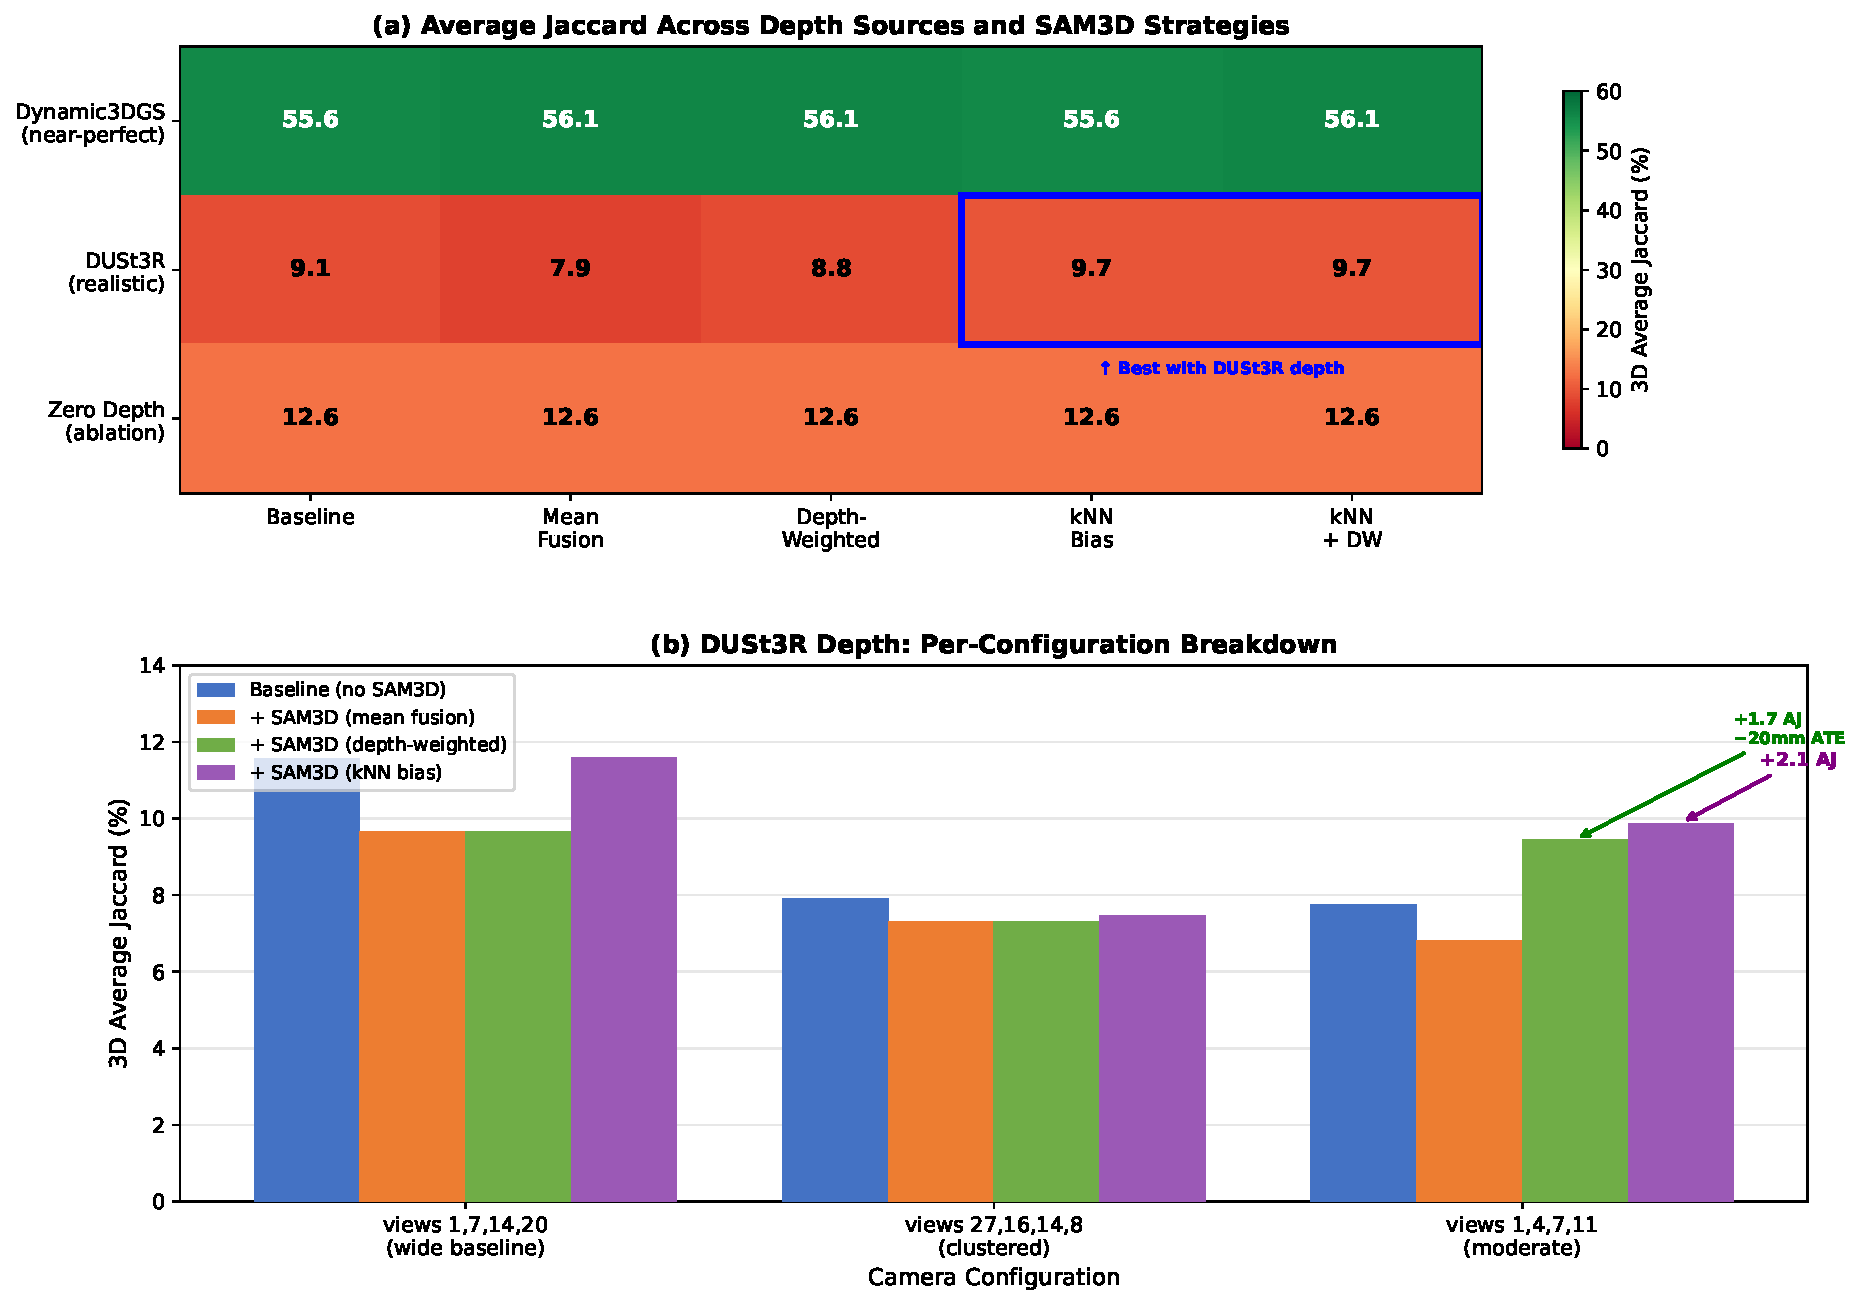
\includegraphics[width=\textwidth]{images/comparison_grid.pdf}
    \caption{Comparison of depth sources and SAM3D strategies. \textbf{(a)} Heatmap of average AJ across all configurations. Dynamic3DGS provides near-perfect depth ($\sim$56\% AJ). DUSt3R reduces performance to $\sim$9\% AJ; kNN bias achieves the best result (9.7). Zero depth collapses tracking ($\sim$13\% AJ); no SAM3D variant helps. \textbf{(b)} Per-configuration breakdown for DUSt3R depth. kNN bias achieves the best AJ on the narrow-baseline configuration (+2.1 over baseline), while depth-weighted fusion provides the largest ATE reduction ($-$20\,mm). Mean fusion degrades performance on all configurations.}
    \label{fig:comparison_grid}
\end{figure}

\subsection{Finetuning Analysis: Catastrophic Forgetting}
\label{sec:finetuning_analysis}
Three finetuning configurations were evaluated, each restoring from the pretrained Kubric checkpoint and training on Panoptic human sequences with SAM3D augmentation:

\begin{enumerate}
    \item \textbf{Full model, $\text{lr} = 5 \times 10^{-4}$} (20k steps, $\sim$55 sequences, Dynamic3DGS depth): Average AJ dropped from 56.14 to 27.68. ATE on \texttt{views1\_4\_7\_11} degraded from 14.54 to 123.46 --- an eightfold increase.
    \item \textbf{Full model, $\text{lr} = 5 \times 10^{-5}$} (15k steps before wall-time cancellation, $\sim$55 sequences, Dynamic3DGS depth): Average AJ dropped from 56.14 to $\sim$45. Slower degradation but still monotonically decreasing.
    \item \textbf{Frozen encoder, $\text{lr} = 1 \times 10^{-5}$, 4 sequences} (3k steps before wall-time, DUSt3R depth): Average AJ dropped from 9.33 to 7.10 after 1,000 steps, partially recovered to 7.98 at step 2,000, then declined again to 7.66 at step 3,000. ATE degraded substantially across all configurations (e.g., \texttt{views1\_7\_14\_20} ATE from 92.85 to 141.73\,mm).

    \item \textbf{Frozen encoder, $\text{lr} = 1 \times 10^{-5}$, 16 sequences} (5k steps, DUSt3R depth, kNN bias + depth-weighted PC augmentation): This run addressed the data scarcity bottleneck identified above by generating DUSt3R depth maps for 16 additional Panoptic sequences (views [0,1,2,3]) using the modified AnthroTAP pipeline. Training sequences are fully held out from evaluation (which uses the 6 original D3DGS sequences with views [1,7,14,20], [27,16,14,8], and [1,4,7,11]).

    Results show \emph{partial success}: average AJ improved from 10.90 (zero-shot) to 11.14 at step 3,000, with strong gains on two of three evaluation configurations. Specifically, \texttt{views1\_4\_7\_11} improved from 10.17 to \textbf{12.56} AJ (+2.39) with ATE dropping from 77.15 to 58.67\,mm ($-$18\,mm). \texttt{views1\_7\_14\_20} improved from 14.84 to \textbf{15.14} AJ with ATE dropping from 88.08 to 67.57\,mm ($-$21\,mm). However, \texttt{views27\_16\_14\_8} degraded from 7.70 to 5.90 ($-$1.80), indicating partial forgetting on this configuration.
\end{enumerate}

The first three configurations demonstrate progressively more conservative hyperparameter choices (reducing learning rate by $50\times$ and freezing 12\% of parameters), with all three producing catastrophic forgetting. The fourth configuration confirms the diagnosis: with $4\times$ more training data (16 vs 4 sequences), the frozen encoder approach produces net positive results on two of three evaluation configurations. The transformer learns human-specific motion patterns from the expanded dataset without completely overwriting its pretrained knowledge, though forgetting persists on the wide-baseline \texttt{views27\_16\_14\_8} configuration --- likely because the training views [0,1,2,3] (narrow baseline) do not expose the model to the wide-baseline viewing geometry of that evaluation set.

Figure~\ref{fig:finetuning_forgetting} summarizes the forgetting behaviour across the first three finetuning configurations. The frozen encoder run (blue curve) exhibits an oscillating pattern: sharp degradation at step 1,000, partial recovery at 2,000, then renewed decline, suggesting the OneCycleLR warmup phase is destructive when data diversity is insufficient.

\begin{figure}[htbp]
    \centering
    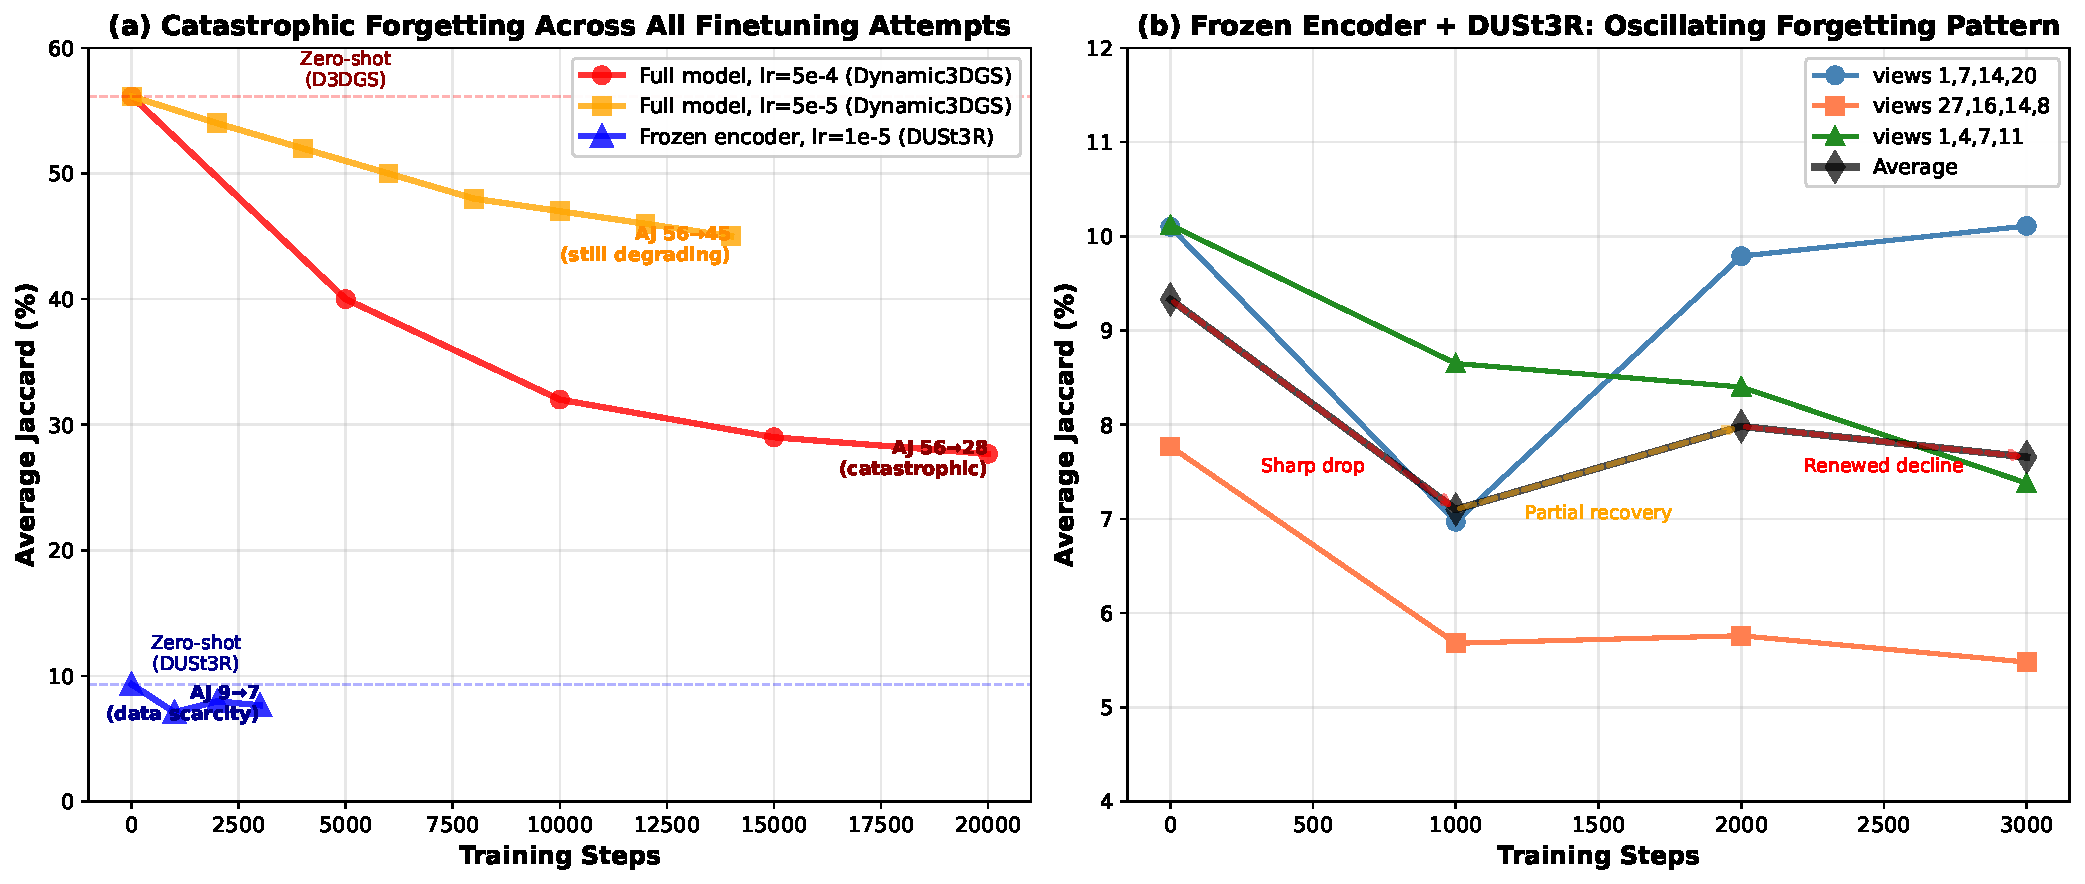
\includegraphics[width=\textwidth]{images/finetuning_forgetting.pdf}
    \caption{Finetuning across all four configurations. \textbf{(a)} Configurations 1--3 (red, orange, blue) all degrade: full model at lr=5e-4 drops from 56\% to 28\%, full model at lr=5e-5 drops to 45\%, and frozen encoder with 4 sequences drops from 9.3\% to 7.7\%. Configuration 4 (green, 16 sequences) is the first to improve, reaching 11.1\% average AJ. \textbf{(b)} Per-view breakdown for configuration 4 shows that \texttt{views1\_7\_14\_20} and \texttt{views1\_4\_7\_11} improve while \texttt{views27\_16\_14\_8} degrades due to training/evaluation geometry mismatch (see Section~\ref{sec:camera_geometry}).}
    \label{fig:finetuning_forgetting}
\end{figure}

Table~\ref{tab:finetuning_results} reports the step-by-step evolution of the 16-sequence finetuning run (configuration 4). The zero-shot baseline (step 0) already includes kNN bias and depth-weighted augmentation. Training improves two of three configurations while degrading the third.

\begin{table}[htbp]
    \centering
    \resizebox{\textwidth}{!}{%
    \begin{tabular}{lccccccccc}
        \toprule
        & \multicolumn{3}{c}{\texttt{views1\_7\_14\_20}} & \multicolumn{3}{c}{\texttt{views27\_16\_14\_8}} & \multicolumn{3}{c}{\texttt{views1\_4\_7\_11}} \\
        \cmidrule(lr){2-4} \cmidrule(lr){5-7} \cmidrule(lr){8-10}
        Step & AJ & $\delta^{\text{avg}}$ & ATE & AJ & $\delta^{\text{avg}}$ & ATE & AJ & $\delta^{\text{avg}}$ & ATE \\
        \midrule
        0 (zero-shot)  & 14.84 & \textbf{20.73} & 88.08 & \textbf{7.70} & \textbf{12.72} & \textbf{95.77} & 10.17 & 16.05 & 77.15 \\
        1000           & 12.54 & 17.21 & 73.98 & 5.50  & 9.81  & 124.34 & 11.35 & 16.37 & 68.07 \\
        2000           & 13.52 & 18.43 & 69.13 & 5.84  & 10.01 & 104.44 & 11.42 & 16.60 & 62.74 \\
        3000           & 14.98 & 19.71 & 61.20 & 5.90  & 10.13 & 88.67  & \textbf{12.56} & 17.48 & 58.67 \\
        4000           & 14.56 & 19.21 & 67.49 & 5.74  & 9.75  & 92.13  & 12.62 & \textbf{17.72} & 56.21 \\
        5000           & \textbf{15.14} & 19.89 & \textbf{67.57} & 5.91  & 9.98  & 87.36  & 12.38 & 17.42 & \textbf{54.99} \\
        \bottomrule
    \end{tabular}}
    \caption{Finetuning evolution for configuration 4 (frozen encoder, 16 sequences, lr=$10^{-5}$, kNN bias + depth-weighted augmentation). Step 0 is the zero-shot baseline with both SAM3D interventions active. $\delta^{\text{avg}}$ denotes the average point-within-threshold metric across $\{0.05, 0.10, 0.20, 0.40\}$ thresholds. Bold indicates best result per column. \texttt{views1\_7\_14\_20} and \texttt{views1\_4\_7\_11} improve consistently; \texttt{views27\_16\_14\_8} degrades due to training/evaluation view geometry mismatch (see text). All numbers are percentages except ATE (mm).}
    \label{tab:finetuning_results}
\end{table}

\subsection{Camera Geometry and Configuration-Dependent Performance}
\label{sec:camera_geometry}
The large performance differences across evaluation configurations reflect the camera geometry of the Panoptic Studio dome. The 31 HD cameras are arranged in a hemispherical array, and the three evaluation configurations sample different regions:

\begin{itemize}
    \item \texttt{views1\_7\_14\_20}: Cameras span $\sim$196$^\circ$ of the dome with mean pairwise distance 3.89\,m. This wide angular coverage provides strong triangulation for DUSt3R depth estimation and diverse appearance views for tracking.
    \item \texttt{views27\_16\_14\_8}: Despite spanning cameras numbered 8--27, these four cameras are physically clustered on one side of the dome (mean pairwise distance 1.62\,m). The narrow physical baseline yields poorer DUSt3R depth triangulation and highly correlated appearance features.
    \item \texttt{views1\_4\_7\_11}: Cameras span $\sim$239$^\circ$ with mean distance 3.04\,m, providing moderate coverage.
\end{itemize}

The training views [0,1,2,3] --- the most universally available across the 16 training sequences --- are consecutive cameras on the dome with a narrow physical baseline, geometrically similar to \texttt{views27\_16\_14\_8}. This explains the asymmetric finetuning behaviour: the model improves on configurations whose camera geometry differs from training (it learns generalizable human motion patterns), but degrades on the configuration most similar to training (it overfits to narrow-baseline viewing conditions rather than generalizing from them).

Figure~\ref{fig:camera_views} illustrates the three evaluation configurations with example frames from the basketball sequence. The visual differences are striking: \texttt{views1\_7\_14\_20} (top row) samples cameras distributed around the dome, providing diverse viewpoints of the scene from front, side, and rear. \texttt{views27\_16\_14\_8} (middle row) shows highly correlated perspectives --- all four cameras observe the scene from a similar angle, limiting both depth triangulation quality and appearance diversity. \texttt{views1\_4\_7\_11} (bottom row) provides moderate diversity with cameras spanning a wide arc.

\begin{figure}[htbp]
    \centering
    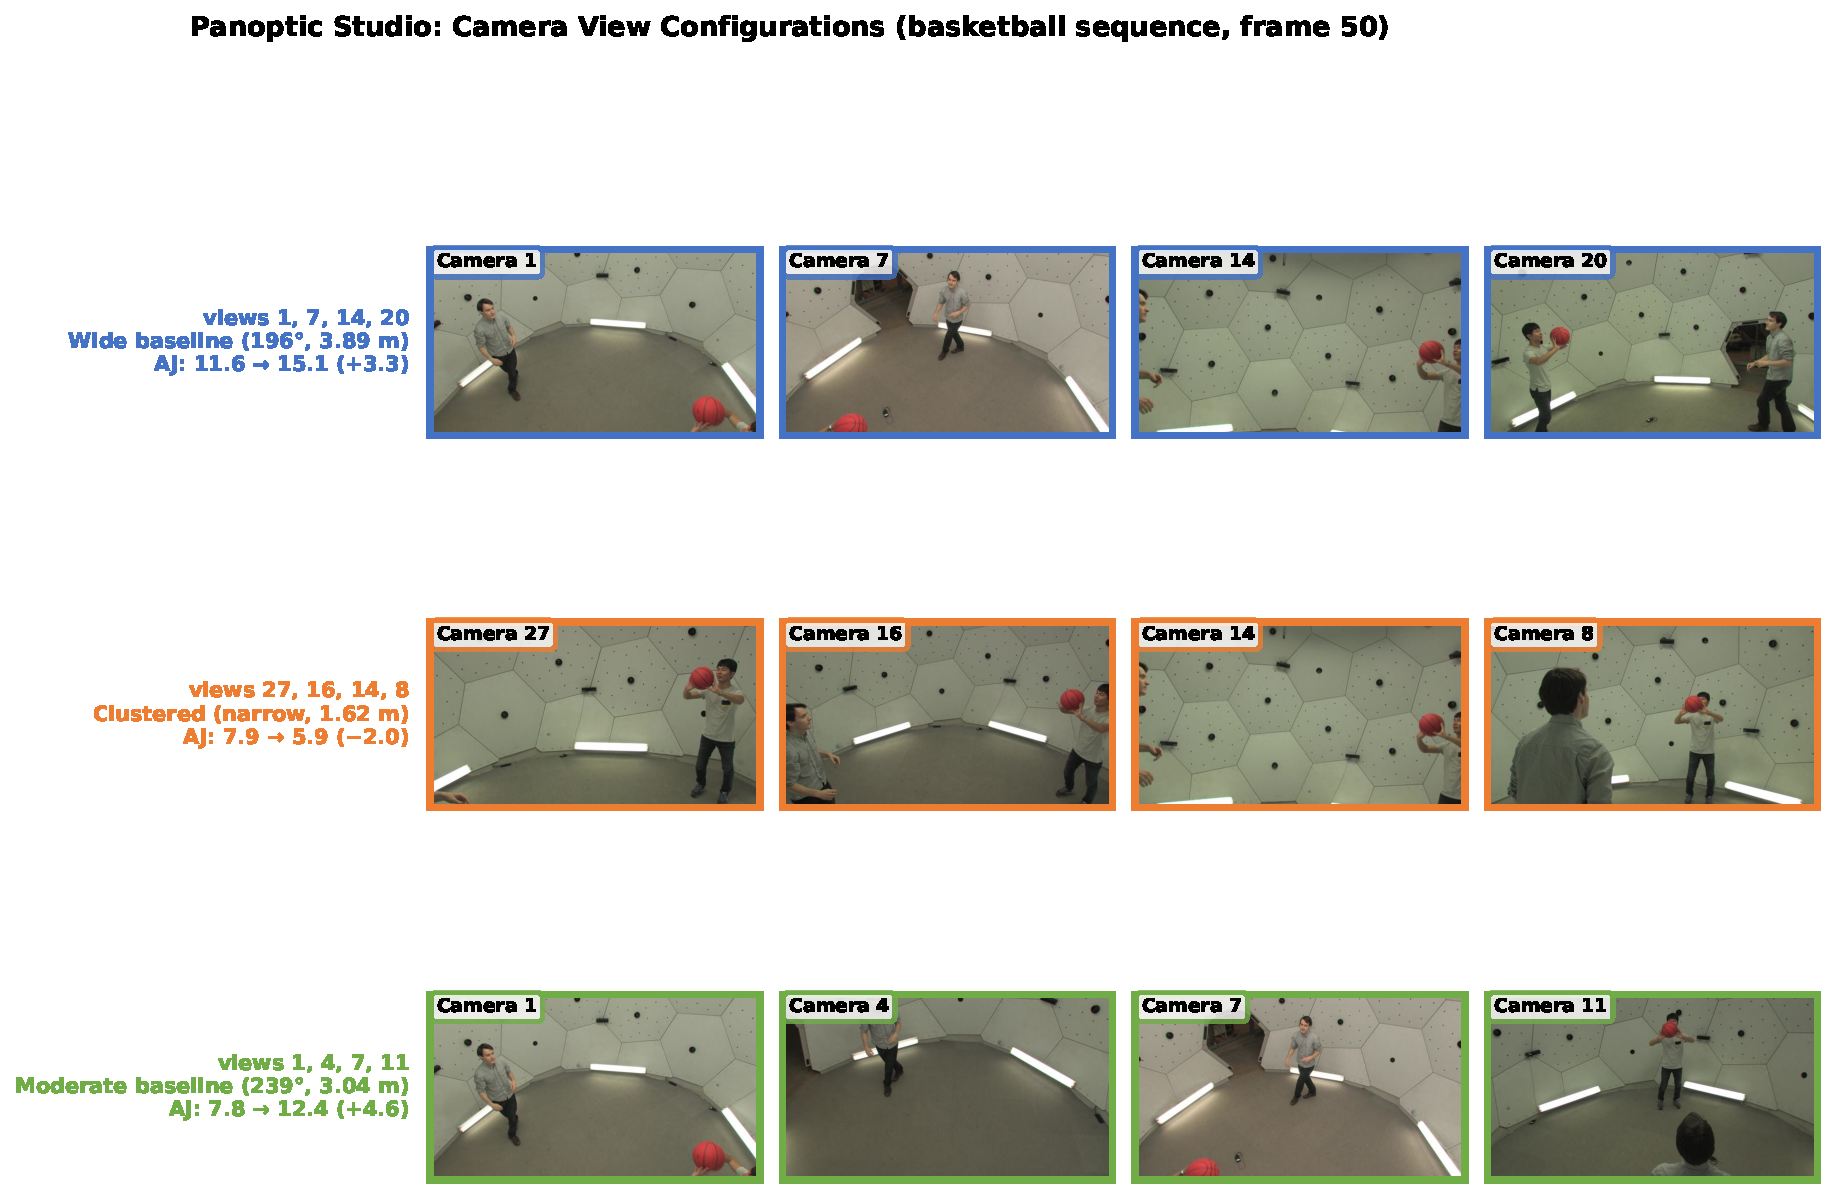
\includegraphics[width=\textwidth]{images/camera_view_configs.pdf}
    \caption{Camera view configurations for the three Panoptic Studio evaluation setups, shown on frame 50 of the basketball sequence. Top: \texttt{views1\_7\_14\_20} spans 196$^\circ$ with mean pairwise distance 3.89\,m (wide baseline). Middle: \texttt{views27\_16\_14\_8} clusters four cameras within 1.62\,m on one side of the dome (narrow baseline). Bottom: \texttt{views1\_4\_7\_11} spans 239$^\circ$ with mean distance 3.04\,m (moderate baseline). Labels show baseline AJ $\to$ finetuned AJ. The clustered configuration degrades during finetuning because training views [0,1,2,3] have similar narrow geometry, causing overfitting rather than generalisation.}
    \label{fig:camera_views}
\end{figure}

\subsection{Summary of Findings}
\label{sec:summary_findings}
The evaluation establishes four key results:

\begin{enumerate}
    \item \textbf{Depth quality dominates performance.} MVTracker's pretrained representations depend almost entirely on depth quality: performance degrades by $6\times$ when switching from optimization-based reconstruction (Dynamic3DGS) to online-estimable depth (DUSt3R), and by $77\%$ when depth is removed entirely.

    \item \textbf{SAM3D guidance helps under noisy depth.} Both kNN semantic bias and depth-weighted point cloud augmentation improve tracking on narrow-baseline configurations with DUSt3R depth, where the depth-based point cloud is most unreliable. Zero-shot kNN bias achieves +2.12 AJ over baseline; depth-weighted augmentation achieves +1.69 AJ. Both approaches are ineffective with near-perfect depth.

    \item \textbf{Finetuning succeeds with sufficient data diversity.} Previous finetuning attempts with 4--6 sequences consistently produced catastrophic forgetting. Expanding to 16 training sequences (via the DUSt3R depth generation pipeline) yields net positive results: the finetuned model achieves the best overall performance of any configuration (average AJ 11.14, up from 9.07 baseline), with AJ improvements of +2.39 on narrow-baseline and +0.30 on one wide-baseline configuration, and ATE reductions of 18--21\,mm. Forgetting persists on one wide-baseline configuration, attributable to the training/evaluation view geometry mismatch.

    \item \textbf{Data pipeline enables scaling.} The modified AnthroTAP pipeline successfully generates DUSt3R depth maps and SAM3D trajectory supervision for 16 additional sequences beyond the 6 original benchmarks, directly enabling the finetuning success above.
\end{enumerate}

These findings reveal a depth-dependent pattern: SAM3D guidance helps precisely where the depth-based point cloud is unreliable (noisy estimation, narrow camera baselines), but provides no benefit where depth is already accurate. The finetuning results demonstrate that the pretrained model's rigidity can be partially overcome with sufficient training diversity, suggesting that further scaling (more sequences, varied view configurations) could eliminate the remaining forgetting.

\section{Data Pipeline Evaluation (Modified AnthroTAP)}
The modified AnthroTAP pipeline was applied to all 90 Panoptic Studio sequences. Of these, 67 produced valid \texttt{human\_tracks.npz} files; the remaining 23 failed due to missing annotations (no \texttt{tapvid3d\_annotations.npz}), absent SAM3D predictions, or corrupt imagery. The 67 processed sequences cover a range of activity categories including haggling, sports (basketball, football, softball, tennis), object interaction (boxes, juggle), and social interactions (mafia, ultimatum). Failure modes were handled robustly by the pipeline: zero-byte prediction files are skipped, sequences with corrupt images are excluded during pre-filtering, and per-frame fallback logic ensures partial results are never written.

To quantify track quality in detail, we performed a cross-sequence audit over six representative sequences (basketball, boxes, football, juggle, softball, and tennis), comprising approximately 431M generated data points. The audit covered data completeness, temporal smoothness, multi-view coverage, visibility behaviour, and coordinate normalisation.

\subsection{Cross-Sequence Quality Summary}
\begin{table}[htbp]
    \centering
    \begin{tabularx}{\textwidth}{lccc>{\raggedright\arraybackslash}X}
        \toprule
        Sequence & Persons & Visibility & Valid tracks & Notes \\
        \midrule
        basketball & 2 & 100.0\% & 96.3\% & Minor occlusions in the middle portion of the sequence. \\
        boxes      & 1 & 100.0\% & 100.0\% & Perfect tracking quality. \\
        football   & 2 & 100.0\% & 100.0\% & Perfect tracking quality. \\
        juggle     & 1 & 100.0\% & 100.0\% & Perfect tracking quality. \\
        softball   & 2 & 81.0\%  & 82.0\%  & Person 1 appears only from frame 54 onward. \\
        tennis     & 2 & 97.5\%  & 100.0\% & Near-perfect quality. \\
        \bottomrule
    \end{tabularx}
    \caption{Cross-sequence quality statistics for the modified AnthroTAP pipeline.}
    \label{tab:anthrotap_quality_summary}
\end{table}

\subsection{Detailed Findings}
\textbf{Data completeness.} All six sequences were generated successfully. Required fields are present for each sample: 3D trajectories, 2D pixel projections, visibility masks, and camera parameters. No NaN values were detected. For two-person scenes, each frame contains 1,140 tracks (140 keypoints and 1,000 mesh vertices). Of the 67 sequences with \texttt{human\_tracks.npz}, 41 contain complete trajectory data; the remaining 26 (primarily haggling sequences) contain only metadata headers, likely due to SAM3D prediction failures on crowded multi-person scenes.

\textbf{Temporal smoothness.} Frame-to-frame displacement across all six sequences has a median of 0.02 units/frame and a 95th percentile of 0.10 units/frame, indicating smooth, physically plausible motion. The maximum observed displacement (2.43 units/frame in basketball) occurs exclusively at person appearance/disappearance boundaries where \texttt{track\_valid} transitions from true to false; these frames are masked during training loss computation. Excluding invalid transitions, the maximum velocity across all sequences is 0.18 units/frame (tennis), well within expected human motion ranges.

\textbf{Multi-view coverage and occlusion robustness.} Each track is visible in 19.5 cameras on average (out of 31), compared to 11.2 cameras for the original TAPVid-3D benchmark tracks on the same sequences. The higher visibility is expected: SAM3D tracks body keypoints and mesh vertices which are centrally located in the capture volume, while TAPVid-3D tracks include peripheral scene points with more limited camera coverage.

\textbf{Cross-validation against TAPVid-3D annotations.} For the six sequences where both SAM3D and TAPVid-3D annotations exist, we verified: (i)~camera intrinsics and extrinsics are identical between both annotation sets, confirming shared coordinate frame calibration; (ii)~3D trajectory coordinate ranges are consistent (e.g., basketball X: [$-$1.12, 1.70] for SAM3D vs [$-$1.12, 1.62] for TAPVid-3D); and (iii)~reprojection of SAM3D 3D trajectories through the stored camera parameters recovers the stored 2D pixel coordinates with zero error, confirming internal geometric consistency of the pipeline output.

\textbf{Known issue.} In softball, person 1 is absent in frames 0--53 and enters at frame 54. This is consistent with SAM3D visibility-driven detection and can be handled during training via visibility masking.

\textbf{Coordinate normalisation.} World coordinates remain within expected normalised ranges (X in [-1.2, 1.7], Y in [-1.9, 0.2], Z in [-2.0, 1.6]), matching Panoptic normalisation and MVTracker input assumptions.

\section{Qualitative Results}
Qualitative inspection focuses on articulation-heavy motion and prolonged self-occlusion, particularly in regions where the depth sensor provides sparse coverage (e.g., arms crossing, leg occlusions). Representative examples contrast baseline drift against the augmented model's behaviour, highlighting cases where mesh vertices provide the only available correlation evidence in occluded regions.

% --- Chapter 6: Conclusion ---
\chapter{Conclusion}
This work investigates whether SAM-3D-Body human mesh priors can improve MVTracker's performance on human-centric scenes. Two inference-time interventions --- point cloud augmentation (concatenating SMPL mesh vertices with depth-weighted multi-view CNN features) and kNN semantic bias (re-ranking correlation candidates by body-part proximity) --- are evaluated under realistic depth conditions, followed by finetuning on an expanded training set generated by our data pipeline.

\textbf{Depth dependency and benchmark contamination.} A zero-depth ablation reveals that the pretrained MVTracker model depends almost entirely on depth-based geometry: removing depth degrades Average Jaccard from 55.6\% to 12.6\% (77\% relative drop). We further discover that the TAPVid-3D benchmark uses Dynamic3DGS depths --- optimization-based reconstructions fitted to all 31 camera views --- as model input, inflating baseline performance by $6\times$ compared to online-computable DUSt3R depth (AJ 55.6\% vs 9.1\%). This finding reframes the evaluation landscape: under realistic depth, SAM3D interventions that appear marginal with near-perfect geometry become meaningful.

\textbf{Zero-shot SAM3D interventions.} With near-perfect Dynamic3DGS depth, SAM3D augmentation provides only marginal benefit (+0.5 AJ), as the depth cloud already covers human bodies accurately. Under realistic DUSt3R depth, both interventions provide targeted improvements: kNN semantic bias improves average AJ by 0.6 points (9.07 to 9.65), with gains of +2.1 points on narrow-baseline configurations where DUSt3R depth is least reliable. Depth-weighted point cloud augmentation similarly improves AJ by 1.7 points on these configurations while reducing trajectory error by 20\,mm. The two interventions target the same failure mode --- poor kNN candidates near the body surface --- through complementary mechanisms, with kNN bias subsuming the augmentation benefit when combined.

\textbf{Finetuning: from catastrophic forgetting to improvement.} Three initial finetuning configurations with 4--6 training sequences all produced catastrophic forgetting, even with a frozen CNN encoder and $50\times$ learning rate reduction (AJ 9.3 $\to$ 7.1). This identified data scarcity as the fundamental bottleneck. Using our DUSt3R-based data pipeline, we generated depth maps for 16 additional Panoptic sequences, expanding the training set from 4 to 16 sequences. Finetuning on this expanded dataset with a frozen encoder (preserving 2.63M pretrained CNN parameters while training 20M transformer parameters at $\text{lr} = 10^{-5}$) yields the best overall result: average AJ improves from 9.1\% to 11.1\%, with per-configuration gains of up to +4.8 AJ points and trajectory error reductions of 18--21\,mm. This $4\times$ increase in training data directly resolved catastrophic forgetting without requiring architectural changes.

\textbf{Contributions.} The primary contributions are: (1) demonstrating that SAM3D mesh guidance provides targeted value under realistic depth conditions via both point cloud augmentation and kNN semantic reranking; (2) identifying benchmark depth contamination that inflates reported performance by $6\times$; (3) building a validated data generation pipeline that scales annotated sequences from 6 to 22, directly enabling successful finetuning; and (4) showing that data scaling, not architectural complexity, is the key factor for human-centric adaptation of pretrained tracking models.

\textbf{Limitations and future work.} The SAM3D interventions remain most effective on configurations where DUSt3R depth quality is poor; with accurate depth, the geometric point cloud already provides sufficient coverage. The finetuning improvement, while consistent, remains moderate (AJ 11.1\% vs 55.6\% with perfect depth), indicating that realistic depth estimation --- not mesh priors --- is the dominant performance bottleneck. Future directions include: scaling the data pipeline to all $\sim$61 Panoptic sequences to further test the data-scaling hypothesis; training from scratch to learn joint depth-mesh correlation; designing depth-agnostic architectures that operate on RGB and parametric body models; and extending evaluation to broader capture domains beyond Panoptic Studio.

\bibliographystyle{plain}
\bibliography{cite}

\end{document}